%%%%%%%%%%%%%%%%%%%%%%%%%%%%%%%%%%%%%%%%%%%%%%%%%%%%%%%%%%%%%%%%%%%%%%%%%%%%%%%%%%%%%%%%%%%%%%%%%%%%%%%
%%													%%
%% 	DIPLOMOVÁ PRÁCE -  Návrh webového administrátorského rozhraní pro platformu GIS.lab			%%
%% 				 Tereza Kulovaná							%%
%%													%%
%% pro formátování využita šablona: http://geo3.fsv.cvut.cz/kurzy/mod/resource/view.php?id=775 	%%
%%													%%
%%%%%%%%%%%%%%%%%%%%%%%%%%%%%%%%%%%%%%%%%%%%%%%%%%%%%%%%%%%%%%%%%%%%%%%%%%%%%%%%%%%%%%%%%%%%%%%%%%%%%%% 

\documentclass[%
  12pt,         			% Velikost základního písma je 12 bodů
  a4paper,      			% Formát papíru je A4
  oneside,       			% Oboustranný tisk
  pdftex,				    % překlad bude proveden programem 'pdftex' do PDF
%%%  draft
]{report}       			% Dokument třídy 'zpráva'
%

\newcommand{\Fbox}[1]{\fbox{\strut#1}}

\usepackage[czech, english]{babel}	% použití češtiny, angličtiny
\usepackage[utf8]{inputenc}		% Kódování zdrojových souborů je UTF8

\usepackage[square,sort,comma,numbers]{natbib}

\usepackage{caption}
\usepackage{subcaption}
\captionsetup{font=small}
\usepackage{enumitem} 
\setlist{leftmargin=*} % bez odsazení

\makeatletter
\setlength{\@fptop}{0pt}
\setlength{\@fpbot}{0pt plus 1fil}
\makeatletter

\usepackage[dvips]{graphicx}   
\usepackage{color}
\usepackage{transparent}
\usepackage{wrapfig}
\usepackage{float} 

\usepackage{cmap}           
\usepackage[T1]{fontenc}    

\usepackage{textcomp}
\usepackage[compact]{titlesec}
\usepackage{amsmath}
\addtolength{\jot}{1em} 

\usepackage{chngcntr}
\counterwithout{footnote}{chapter}

\usepackage{acronym}

\usepackage[
    unicode,                
    breaklinks=true,        
    hypertexnames=false,
    colorlinks=true, % true for print version
    citecolor=black,
    filecolor=black,
    linkcolor=black,
    urlcolor=black
]{hyperref}         

\usepackage{url}
\usepackage{fancyhdr}
%\usepackage{algorithmic}
\usepackage{algorithm}
\usepackage{algcompatible}
\renewcommand{\ALG@name}{Pseudokód}% Update algorithm name
\def\ALG@name{Pseudokód}

\usepackage{dirtree}
\usepackage{booktabs}
\usepackage{graphicx}
\usepackage[table,xcdraw]{xcolor}

\usepackage[
  cvutstyle,          
  diploma           
]{thesiscvut}


\newif\ifweb
\ifx\ifHtml\undefined % Mimo HTML.
    \webfalse
\else % V HTML.
    \webtrue
\fi 

\renewcommand{\figurename}{Obrázek}
\def\figurename{Obrázek}

%%%%%%%%%%%%%%%%%%%%%%%%%%%%%%%%%%%%%%%%%%%%%%%%%%%%%%%%%%%%%%%%%
%%%%%%%%%%% Definice informací o dokumentu  %%%%%%%%%%%%%%%%%%%%%
%%%%%%%%%%%%%%%%%%%%%%%%%%%%%%%%%%%%%%%%%%%%%%%%%%%%%%%%%%%%%%%%%

%% Název práce
\nazev{Rozšíření zásuvného modulu QGIS pro zpracování GTFS o vizualizaci tarifních pásem PID }
{QGIS GTFS Plugin extension with visualization of PID tariff zones }

%% Jméno a příjmení autora
\autor{Bc.~Martin}{Kouba}

%% Jméno a příjmení vedoucího práce včetně titulů
\garant{Ing.~Martin~Landa,~Ph.D.}

%% Označení programu studia
\programstudia{Geodézie a~kartografie}{}

%% Označení oboru studia
\oborstudia{Geomatika}{}

%% Označení ústavu
\ustav{Katedra geomatiky}{}

%% Rok obhajoby
\rok{2021}

%Mesic obhajoby
\mesic{červen}

%% Místo obhajoby

\misto{Praha}

%% Abstrakt
%\abstrakt {slova}

%% Klíčová slova
\klicovaslova
{Python, QGIS, zásuvný modul, GTFS, PyQGIS}
{Python, QGIS, plugin, GTFS, PyQGIS}

%%%%%%%%%%%%%%%%%%%%%%%%%%%%%%%%%%%%%%%%%%%%%%%%%%%%%%%%%%%%%%%%%%%%%%%%

%%%%%%%%%%%%%%%%%%%%%%%%%%%%%%%%%%%%%%%%%%%%%%%%%%%%%%%%%%%%%%%%%%%%%%%%
%% Nastavení polí ve Vlastnostech dokumentu PDF
%%%%%%%%%%%%%%%%%%%%%%%%%%%%%%%%%%%%%%%%%%%%%%%%%%%%%%%%%%%%%%%%%%%%%%%%
\nastavenipdf
%%%%%%%%%%%%%%%%%%%%%%%%%%%%%%%%%%%%%%%%%%%%%%%%%%%%%%%%%%%%%%%%%%%%%%%

%%% Začátek dokumentu
\begin{document}

\catcode`\-=12  % pro vypnuti aktivniho znaku '-' pouzivaneho napr. v \cline 

% aktivace záhlaví
\zahlavi

% předefinování vzhledu záhlaví
\renewcommand{\chaptermark}[1]{%
	\markboth{\MakeUppercase
	{%
	\thechapter.%
	\ #1}}{}}

% Vysázení přebalu práce
%\vytvorobalku

% Vysázení titulní stránky práce
\vytvortitulku

% Vysázení listu zadani
\stranka{}%
	{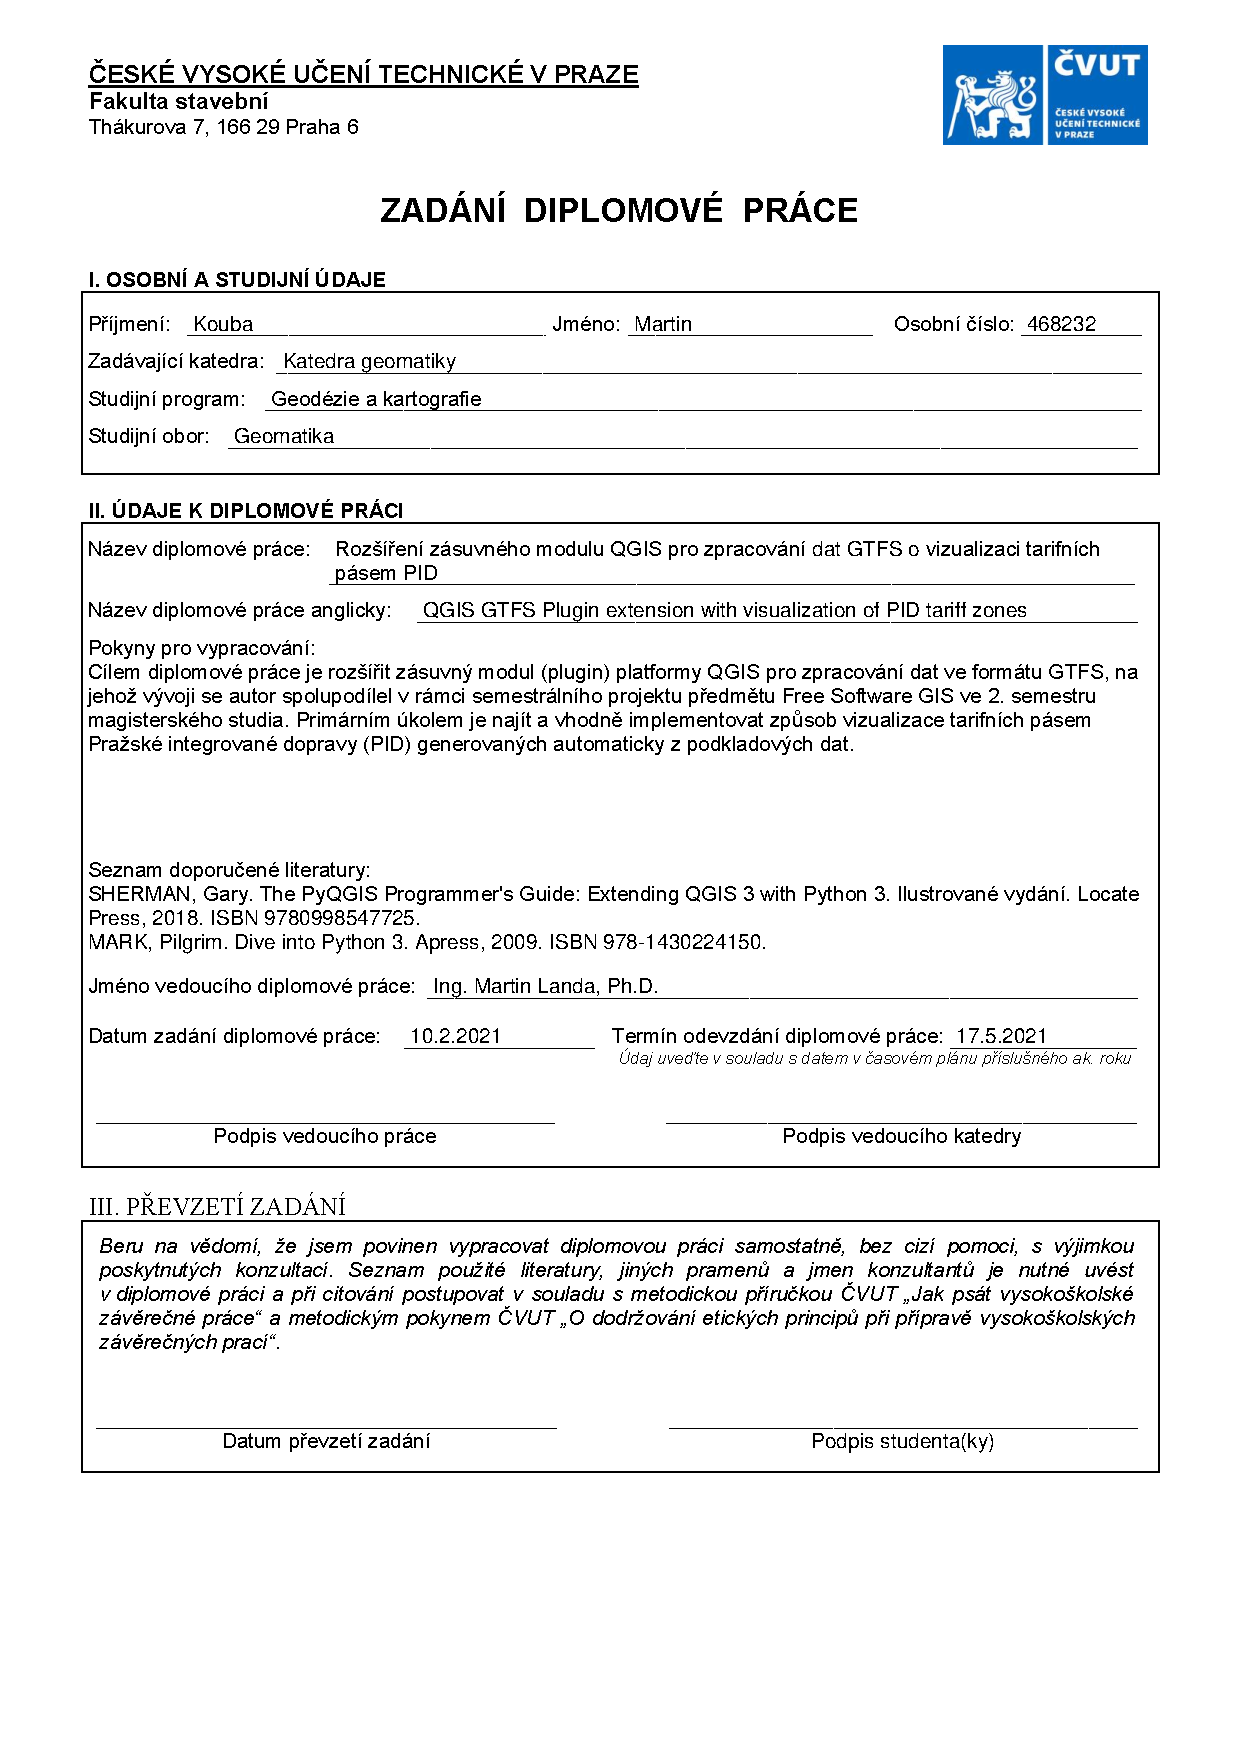
\includegraphics[scale=0.7]{../zadani/zadanidp.pdf}}%\sffamily\Huge\centering\ }%ZDE VLOŽIT LIST ZADÁNÍ}%
	%{\sffamily\centering Z~důvodu správného číslování stránek}

% Vysázení stránky s abstraktem
\vytvorabstrakt

% Vysázení prohlaseni o samostatnosti
\vytvorprohlaseni

% Vysázení poděkování
\stranka{%nahore
       }{%uprostred
       }{%dole
       \sffamily
	\begin{flushleft}
		\large
		\MakeUppercase{Poděkování}
	\end{flushleft}
	\vspace{1em}
		%\noindent
	\par\hspace{2ex}
	{Tímto bych chtěl poděkovat panu Ing. Martinu Landovi, Ph.D. za pomoc při …………………………………
	Zvlášť bych chtěl poděkovat celé své rodině …………………………………………
}
}

% Vysázení obsahu
\obsah

% Vysázení seznamu obrázků
\seznamobrazku

% Vysázení seznamu tabulek
\seznamtabulek

% jednotlivé kapitoly
\chapter*{Úvod}
\addcontentsline{toc}{chapter}{Úvod}
\markboth{ÚVOD}{}
\label{0-uvod}

Pro cestování po Praze a okolí je často nejlepší volbou použít veřejnou dopravu.
Tu zahrnuje metro, tramvaje, železnici, městské a příměstské autobusové linky,
%% ML: druha veta je nesrozumitelna, prepiste ji (a rozdelte do dvou)
lanovou dráhu na Petřín a také některé přívozy. Celý tento systém se nazývá 
Pražská integrovaná doprava, který je postupně integrován společnými přepravními
a tarifními podmínkami a jednotným dopravním řešením včetně koordinace jízdních řádů.

Systém Pražské integrované dopravy je rozdělen do dvanácti tarifních pásem, pro
které platí různé jízdní doklady. Rozlohově jsou po celé Praze, na většině
Středočeského kraje a dokonce i na částech Plzeňského a Ústeckého kraje, či na Vysočině.
%% ML: je uvedeno
Více o systému Pražské integrované dopravy je v kapitole \ref{3-teorie-pid}.

%% ML: slova "zatim" bych vynechal
Tarifní pásma Pražské integrované dopravy jsou zatím modelována manuálně a nejsou
%% ML: a jejich tvorba neni nikterak ...
%% ML: uvod ma byt v minulem case
nikterak zautomatizována. Cílem této diplomové práce bude vytvořit postup pro
automatické vyhotovení exaktního modelu tarifních pásem a co nejvíce se přiblížit k jejich
%% ML: alternativnim -> druhotnym
oficiální podobě vydávaným organizací ROPID. Alternativním cílem je vytvořit schématický model, který nesplňuje tolik
pravidel pro tvorbu tarifních pásem, ale má informační hodnotu pro mapy menších měřítek
například pro různé plánky Pražské integrované dopravy. V postupu se bude využívat GTFS 
dataset, o kterém se mimo jiné píše v kapitole \ref{2-teorie-gtfs}.

%% ML: Misto "zaverecna" je presnejsi uvadet "diplomova"
Tato závěrečná práce navazuje na vývoj zásuvného modulu
%% ML: vetu prepiste: "u ktereho byla zapocata tvorba" nezni prilis pekne
v softwaru QGIS, u kterého byla započata tvorba v předmětu Free software GIS
v 5. semestru magisterského studia s mými spolužáky Adrianou Brezničanovou a Jaroslavem
%% ML: "technologie tvorby" ?
Zemanem. O softwaru QGIS a dalších technologiích tvorby se pojednává v kapitole 
\ref{4-technologie}.

V poslední kapitole \ref{5-postup} je popsán postup tvorby rozšíření zásuvného modulu.
%% ML: posledni vetu prepiste "do kterych se musel vydat" zni opravdu kostrbate...
Zahrnuje i několik slepých uliček postupu, do kterých se muselo vydat kvůli zjištění
vhodnějšího postupu.    




\chapter{Rešerše}
\label{0-reserse}

Tarifní pásma Pražské integrované dopravy jsou mimo jiné publikována jako shapefile 
\footnote{formát vektorového datového úložiště Esri pro ukládání umístění,
tvaru a atributů geografických prvků \cite{shapefile}}
na portálu \textit{opendata hlavního města Prahy} \cite{opendata}. Tento shapefile
obsahuje vektorové vrstvy polygonů.

První myšlenkou, jak se přiblížit k takovým polygonům bylo vytvoření linií mezi jednotlivými zastávkami.
K tomu slouží takzvaná triangulace, která vytvoří trojúhelníky bezi body, kde uvnitř těchto trojuhelníků  
už neleží žádné body a každý trojúhelník má vždy společnou jednu hranu. 

Takové triangulace se používají v kartografii, tak v GIS, v Dálkovém průzkumu země,
počítačové grafice, při analýze vlastností a struktury materiálů, plánování pohybu robotů
nebo při modelování přírodních jevů. \cite{bayer-delaunay}

Existuje více druhů triangulací, které využívají vždy jinou metodu konstrukce
a mají rozdílný výpočetní stupeň složitosti. 

Hladová (Greedy) triangulace se snaží vytvářet trojúhelníky s nejkratšími stranami,
které nesplňují žádnou speciální geometrickou podmínku. Její realizace je jednoduchá,
avšak důsledek toho jsou často tvarově nepěkné nebo nevhodné trojúhelníky. Má velkou výpočetní
složitost \(O(n^3)\), lze optimalizovat na \(O(n^2 \log(n))\) a v kartografii se 
nepříliš používá. \cite{vanicek}

\begin{figure}[H] \centering
    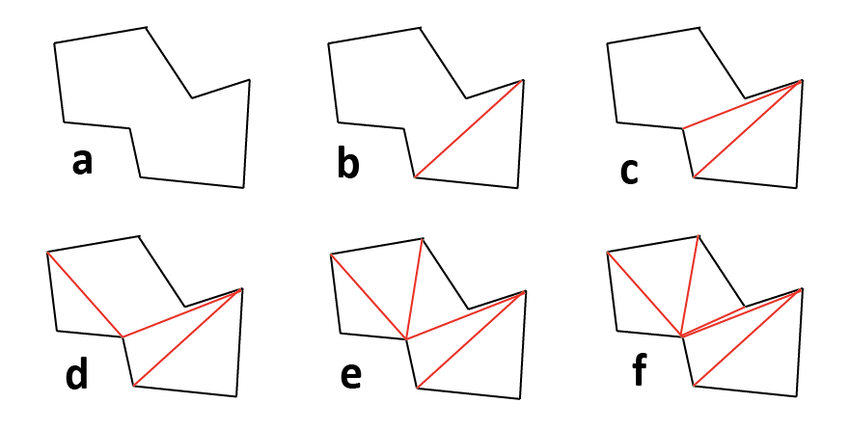
\includegraphics[width=400pt]{./pictures/triangulace-greedy.png}
    \caption[Ilustrace Greedy triangulace]{Ilustrace Greedy triangulace \cite{triangulace-greedy}}
	\label{fig:triangulace-greedy}              
\end{figure}

Další triangulací je tzv. Delaunay triangulace, která je nejčastěji používaná.
Delaunay triangulací se rozumí vytváření liniových spojnic bodů mez jednotlivými body, které si jsou sobě nejblíž,
za pomocí opsaných kružnic. Delaunay triangulace má několik vlastností. Jednou z nich je například,
že uvnitř kružnice k opsané libovolnému trojúhelníku neleží žádný jiný bod.
Zároveň Delaunay triangulace je jednoznačná, pokud žádné čtyři body neleží na kružnici.
Na rozdíl od Greedy triangulace nehodnotí kritérium délky hran. Díky maximalizaci minimálních
úhlů vytváří takové trojúhelníky, které se nejvíc blíží k rovnostranným trojúhelníkům, 
což znamená, že se snaží eliminovat trojúhelníky, které jsou ostroúhlé.

Pro výtváření konstrukce Delaunay triangulace jsou k dispozici různé algoritmy: lokální prohazování, 
inkrementální konstrukce, inkrementální vkládání, rozděl a panuj nebo sweep line. \cite{bayer-delaunay}

\begin{figure}[H] \centering
    
\includegraphics[width=280pt]{./pictures/triangulace-delaunay.png}
    \caption[Ilustrace Delaunay triangulace]{Ilustrace Delaunay triangulace \cite{triangulace-delaunay}}
	\label{fig:triangulace-delaunay}              
\end{figure}

Poté existuje triangulace s minimální hmotností (anglicky Minimum Weight Triangulation, zkráceně MWT),
která má minimální celkovou délku hran. MWT je nejlepší triangulace pro interpolaci trojrozměrných oblastí,
tudíž se pro tvorbu 2D tarifních pásem úplně nehodí.

% Konvexní obálka - definice, metody konstrukce

% Konkávní obálka - definice, metody konstrukce

Tarifní pásma zasahují tam, kde nejsou žádné zastávky. Pro takové vyplnění plochy
mezi zastávkami a pro místa, kde zastávky nejsou (většinou na krajích zón) není triangulace, konvexní nebo konkávní 
obálka úplně vhodná. Pro takový problém bylo další myšlenkou použít teselaci, což je vyplnění roviny pomocí jednoho
nebo více geometrických útvarů vzájemně spojených, bez překrývú a mezer. Triangulace, konvexní nebo konkávní 
obálka se mohou hodit při dalších krocích výpočtu.

Nejpoužívanější teselací v oblastí GIS je Voronoi diagram, někdy nazývána Voroného teselace, Voroného dekompozice,
Thiessenovy polygony nebo Dirichletova teselace, což je způsob rozkladu 
metrického prostoru určený vzdálenostmi k dané nespojité množině bodů v prostoru.
V našem případě se bude řešit Voronoi diagram ve 2D prostoru, tedy v rovině.

Takže na vstupu Voronoi diagramu je nějaká množina bodů a výstupem je Voronoi diagram, 
což představuje takovou množinu buněk, pro které bude platit, že každý bod
\textit{q} nálěžící množině \textit{V(p\textsubscript{i})} je blíže k bodu
\textit{p\textsubscript{i}} než k jakémukoliv
bodu \textit{p\textsubscript{j}} náležící množině \textit{P}.  \cite{bayer-voronoi}

Pro lepší chápání Voronoi diagramů je potřeba si vysvětlit její terminologii.
Vstupní množinu bodů nazýváme generátory, každý bod generuje jednu Voronoi buňku. V 
terminologii GIS se hovoří o tzv. Voronoi polygony. Tyto Voronoi buňky jsou tvořeny hranami,
které spojují dva Voronoi vrcholy. Dohromady tyto Voronoi buňky tvoří Voronoi diagram.  

\begin{figure}[H] \centering
    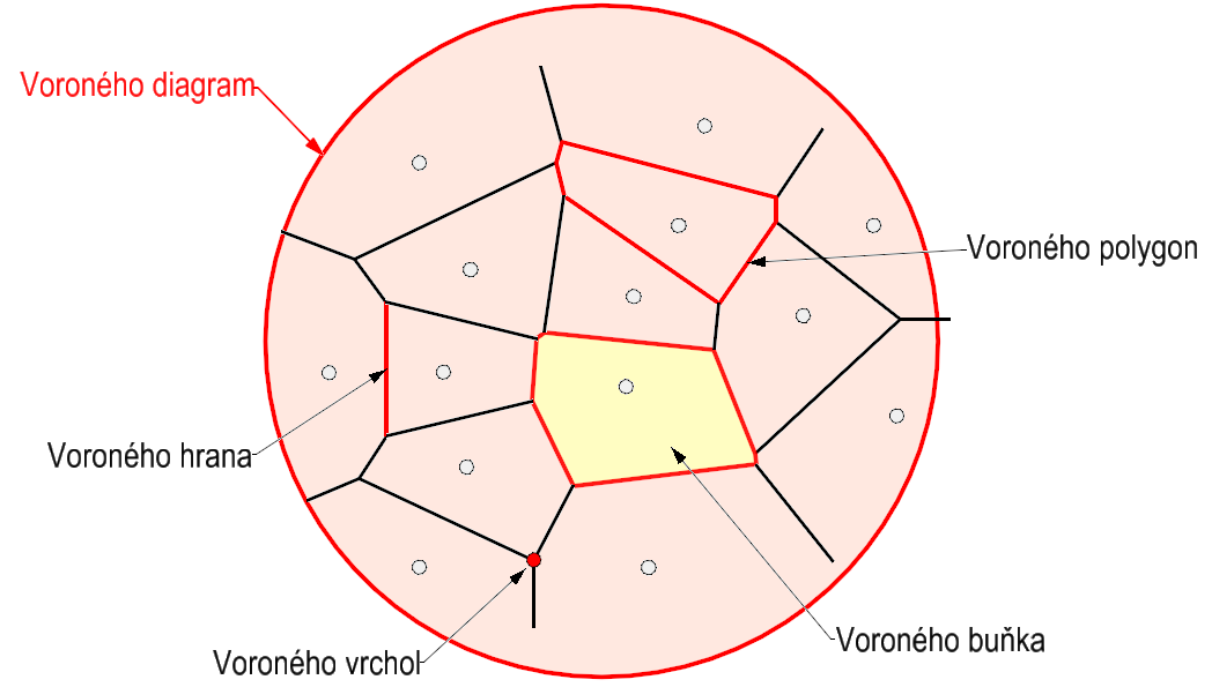
\includegraphics[width=400pt]{./pictures/bayer-voronoi-terminologie.png}
    \caption[Terminologie Voronoi diagramu]{Terminologie Voronoi diagramu \cite{bayer-voronoi}}
	\label{fig:bayer-voronoi-terminologie}              
\end{figure}

Voronoi diagramy mají své vlastnosti, které jsou důležité pro jejich tvorbu. V následujících
odrážkách jsou doslovně citována jejih znění z prezentace pana doc. Ing. Tomáše Bayera, Ph.D.

\begin{itemize}
\item Voronoi diagram \textit{V(P)} je planárním grafem.
\item Vrchol q Voronoi buňky \textit{\{V(p\textsubscript{i})} je průnikem 3 hran, právě když je \textit{V(P)} nedegenerovaný.
\item Pokud \textit{p\textsubscript{i}} náležící \textit{H(P)}, pak je \textit{V(p\textsubscript{i})}  otevřený. 
\item Pro každý bod \textit{p\textsubscript{i} náležící P} je \textit{V(P)} konvexní. 
\item Bod \textit{p\textsubscript{i}} je nejbližším bodem bodu \textit{p}
jestliže \textit{p} náleží \textit{\{V(p\textsubscript{i})}.
\item Každá strana \textit{q\textsubscript{i}q\textsubscript{j}}, \(i \neq j\),
je sdílena právě dvěma sousedními buňkami \textit{V(p)}. 
\item Bod q je vrcholem \textit{V(p)}, pokud existuje kružnice \textit{k(q,r)} procházející třemi
nebo více generátory \textit{p\textsubscript{i}}, \textit{p\textsubscript{j}},
\textit{p\textsubscript{k}}, a neobsahuje žádný další bod P (spojitost s \textit{DT(P)}). 
\item Kružnici \textit{k(q,r)} označujeme jako největší prázdnou kružnici ze všech prázdných kružnic se středem v bodě \textit{q}. 
\item Průměrné množství Voronoi hran ve Voronoi polygonu nepřekročí hodnotu 6. 
\item Vztah mezi počtem bodů \textit{n}, počtem hran \textit{n\textsubscript{h}}
a počtem trojúhelníků \textit{n\textsubscript{t}} teselace \textit{V(P)}:
\[ n_h \leq 3n-6\]
\[ n_t \leq 2n−5\]
\item Voronoi diagram \textit{V(P)} představuje ortografickou projekci stěn
mnohostěnu tvořeného průsečnicemi všech polorovin \textit{A\textsubscript{i}} do roviny \textit{xy}. 
\item Nechť bod \textit{p\textsubscript{i}\textsuperscript{*}} i představuje
ortografický průmět bodu \textit{p\textsubscript{i}} na povrch paraboloidu daného rovnicí:
\[ z = x^2 + y^2 \]
   
\end{itemize}

\begin{figure}[H] \centering
    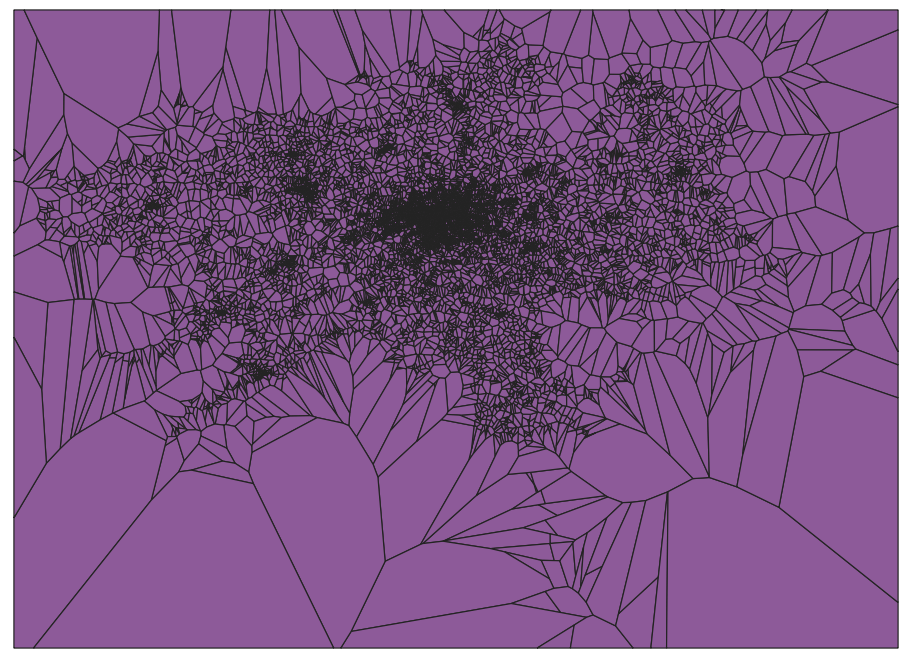
\includegraphics[width=400pt]{./pictures/voronoi.png}
    \caption[Voroného polygony]{Voroného polygony}
	\label{fig:voronoi}              
\end{figure}   

Voronoi diagram má jistý vztah s Delaunay triangulací. Hraniční vstupní body
Voronoi diagramu po spojení Delaunay triangulací tvoří konvexní obálku.
Středy kružnic opsaných trojúhelníků Delaunay triangulace představují úzlové body
Voronoi diagramu.

Pro konstrukci Voronoi diagramu existují různé metody. Konstrukce lze v praxi tvořit přímo nebo nepřímo.
Pro přímou konstrukci jsou tu metody Inkrementální konstrukce, Sweep line algoritmus a
Rozděl a panuj. Nepřímá konstrukce je vytvářena přes Delaunay triangulaci skrz spojení středů
kružnic opsaných trojúhelníků a bývá nejpoužívanější. 

Využití Voronoi diagramů v oblasti GIS je široké. Například tzv. poštovní problém
pomáhá při návrhu nových supermarkétů, stanic MHD či polohy nových nemocnic.
Další využití jsou například nalezení všech sousedů, převod bodových údajů na plošné
nebo klasifikace dat.

 
\chapter{GTFS}
\label{2-teorie-gtfs}

General Transit Feed Specification, zkráceně GTFS, je dokument, který definuje
obecný formát pro jízdní řády veřejné dopravy a příbuzné geografické informace.
GTFS „feeds“ umožňují veřejným dopravním agenturám zveřejňovat svá přepravní
data a vývojářům psát aplikace, které tato data spotřebovávají interoperabilním
způsobem neboli vícesystémovým mezinárodním provozuschopným způsobem. \cite{gtfs-info}

\section{Historie GTFS}
V Portlandu ve státě Oregon v USA se společnost TriMet pokusila jako jedna z prvních 
řešit problém s plánováním tranzitní dopravy pomocí otevřených dat sdílených širokou veřejností.
V roce 2005 společnost TriMet oslovila společnost Google s dotazem, zda mají nějaké plány
na začlenění tranzitní dopravy do svých plánovačů výletů na základě veřejných údajů TriMet.
Google jim kladně odpověděl a spojily síly s implementací jednoho z prvních plánovačů výletů v Portlandu.

Jedním z prvních problémů, kterým TriMet a Google čelily, byl problém udržitelných dat
- pro zajištění kvalitních cest by plánovač cest potřeboval přepravní řád, 
trasu a údaje o zastávkách v elektronickém formátu, který by byl neustále aktuální. 
Společnost TriMet ve spolupráci se společností Google naformátovala svá přepravní 
data do snadno udržovatelného a spotřebního formátu, který lze importovat do Map Google. 
Tento formát dat přepravy se stal známým jako Specifikace zdroje Google Transit (anglicky
Google Transit Feed Specification (GTFS)). 
V roce 2005 byla tato služba plánování cesty spuštěna jako Google Transit.

Od tohoto roku se GTFS stal nejpopulárnějším datovým formátem pro přepravní služby na světě. 
Spousta agentur se rozhodla sdílet své GTFS údaje s veřejností, zatímco některé agentury 
zůstaly zdrženlivé a přístup k datům nechaly jen některým partnerům. Ke 2. prosinci 2019
uvádí OpenMobilityData 1233 poskytovatelů s veřejně přístupnými kanály GTFS,
z nichž 465 je ve Spojených státech. 

V důsledku inovací vývojářů třetích stran jsou data GTFS nyní využívána různými softwarovými aplikacemi
třetích stran k mnoha různým účelům, včetně plánování výletů, map, vytváření jízdních řádů, mobilních dat,
vizualizace, přístupnosti, analytických nástrojů pro plánování a informační systémy v reálném čase.
V roce 2010 byl název formátu GTFS změněn na General Transit Feed Specification,
aby přesně reprezentoval jeho použití v mnoha různých aplikacích mimo produkty Google. \cite{transitwiki} 
 
% doplnit něco o historii GTFS 

\section{GTFS dataset}
GTFS \uv{feed} nebo lépe jako GTFS dataset\footnote{kolekce dat, která by měla být publikována na permanentní URL adrese}
je ZIP soubor, který obsahuje CSV soubory.

CSV, \textit{Comma-separated values}, v překladu \textit{hodnoty oddělené čárkami}, je jednoduchý 
souborový formát určený pro výměnu tabulkových dat. Data jsou oddělována „oddělovačem“.
Ačkoli podle definice by měl být formát oddělen čárkami, oddělovač může být prakticky cokoli. 
Nejčastějšími oddělovači jsou právě čárky, středníky nebo mezery. CSV soubor se 
může upravovat v jakémkoliv textovém editoru.

\begin{figure}[H] \centering
    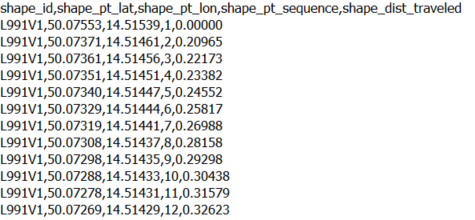
\includegraphics[width=250pt]{./pictures/ukazka-csv.PNG}
    \caption[Ukázka CSV formátu ze souboru shapes.txt]{Ukázka CSV formátu ze souboru shapes.txt}
	\label{fig:ukazka-csv}              
\end{figure}

V GTFS datasetu může být v současné době až 17 CSV souborů v textové podobě. Slovem \uv{může} je myšleno to,
že některé CSV soubory jsou požadované či podmíněně požadované a jiné volitelné.
Jaké CSV soubory obsahuje dataset záleží na konkrétním dopravním systému, který
tento dataset vytváří.

Termín \uv{požadované} znamená, že daný CSV soubor se musí nacházet v GTFS datasetu nebo dané pole
se musí nacházet v CSV souboru a v tomto poli musí být uvedena hodnota pro každý záznam. 

%přidat referenci na podmínky?
Termín \uv{podmíněně} požadované" znamená, že daný CSV soubor nebo pole je vyžadován za určitých podmínek, 
které jsou uvedeny v popisu souboru nebo pole. Mimo tyto podmínky je tento soubor nebo pole volitelný.

Termín \uv{volitelné} znamená, že daný CSV soubor nebo pole může být vynecháno. V případě zahrnutí 
volitelného pole mohou být některé položky prázdné řetězce, což je ekvivalentní s prázdným
polem.

V následující tabulce \ref{table:csv-soubory} jsou přehledně zobrazeny všechny CSV soubory,
které v současnosti v GTFS datasetu mohou být.

\newcolumntype{s}{>{\centering\arraybackslash\columncolor[HTML]{CCFFCC}} m{5cm}}
\newcolumntype{v}{>{\centering\arraybackslash\columncolor[HTML]{C4FFFD}} m{5cm}}

\begin{table}[h!]
\begin{center}
\begin{tabular}{ |s|v| } 
  \hline
  požadované/podmíněně požadované & volitelné \\ 
  \hline
  agency.txt & fare\_attributes.txt \\ 
  stops.txt & fare\_rules.txt \\ 
  routes.txt & shapes.txt \\
  trips.txt & frequencies.txt \\
  stop\_times.txt & transfers.txt \\
  calendar.txt & pathways.txt \\
  calendar\_dates.txt & levels.txt \\ 
  feed\_info.txt & translations.txt \\
  - & attributions.txt \\ 
  \hline      
\end{tabular}
\end{center}
\caption{Seznam CSV souborů v GTFS datasetu}
\label{table:csv-soubory}
\end{table}

Každý CSV soubor v GTFS datasetu má v prvním řádku názvy polí, do kterých je tento
soubor rozřazen. Jednotlivá pole mají různý datové typy, které jsou barva, kód měny, 
datum, email, enum (výčet), ID, kód jazyka, zeměpisná délka, zeměpisná šířka,
nezáporné číslo s plovoucí desetinnou čárkou, nezáporné celé číslo, telefonní číslo,
čas, text, časové pásmo a URL adresa.

Jedno z nejdůležitějších polí je pole s datovým typem ID, což je hodnota jednoznačně určující každý záznam.
Právě tento datový typ umožňuje propojení jednotlivých CSV souborů mezi sebou. ID může být
sekvence libovolných UTF-8 znaků. Pole s datovým typem ID se označují nakonci názvu s
\uv{\_id}. Na následujícím obrázku \ref{fig:GTFS-diagram} je toto propojení zobrazeno pomocí diagramu.

%přidat referenci na podmínky?
Na obrázku \ref{fig:GTFS-diagram} je taktéž tučně zobrazeno, které pole v daném CSV souboru
jsou požadované, podmíněně požadované nebo volitelné. 

\begin{figure}[H] \centering
    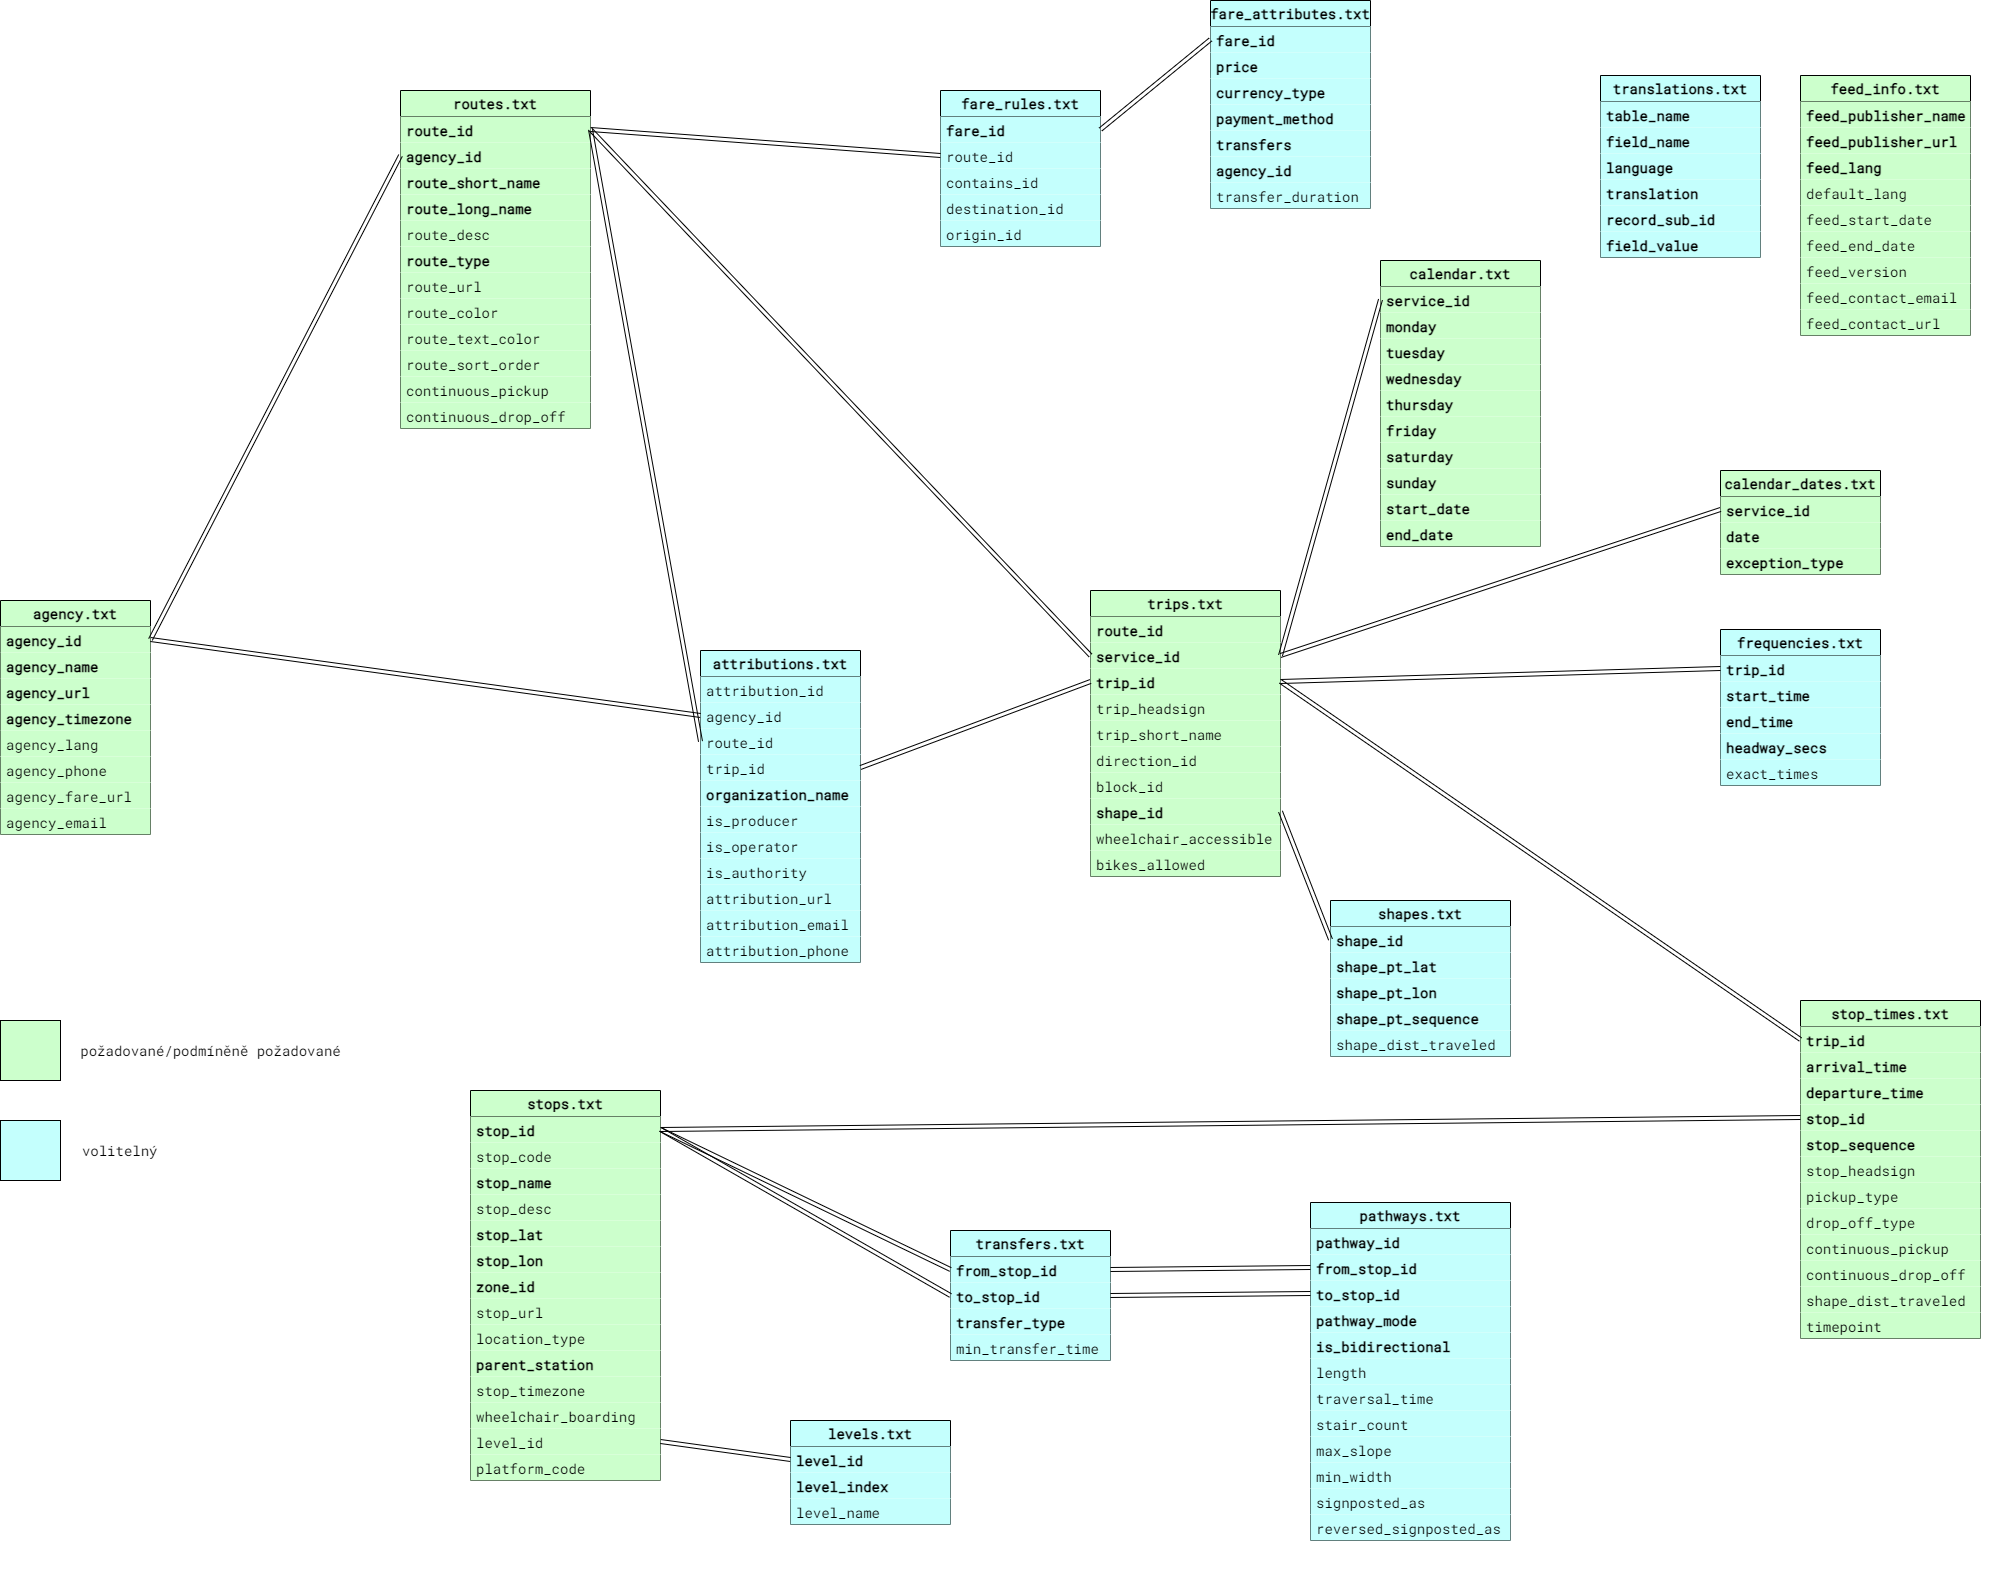
\includegraphics[width=400pt]{./pictures/GTFS-diagram.PNG}
    \caption[Diagram GTFS datasetu]{Diagram GTFS datasetu}
	\label{fig:GTFS-diagram}              
\end{figure}

Pro moji diplomovou práci byly dále důležité datové typy jako zeměpisná délka a zeměpisná šířka,
které již podle názvu obsahují zeměpisnou délku a šířku v souřadnicovém systému WGS84, barva zakódovaná 
jako šestimístné hexadecimální číslo, nezáporné číslo s plovoucí desetinnou čárkou a nezáporné celé číslo
nebo enum, což jsou předem definované konstanty.

\subsection{Soubor stops.txt}
\label{stops.txt}
Soubor \textit{stops.txt} se skládá ze 14 polí, z čehož 6 polí je požadovaných nebo podmíněně požadovaných 
a zbytek volitelných. Samotný soubor je požadovaný a měl by se nacházet v každém GTFS datasetu.

Prvním polem je vždy zpravidla \textit{stop\_id}, které je požadované a má datový typ ID.
Tato hodnota jednoznačně určuje každou zastávku. Pro PID\_GTFS, což je GTFS dataset Pražské integrované dopravy,
se pole \textit{stop\_id} skládá z kombinace písmen a čísel v souvislosti s typem spoje.

Druhým polem je volitelné pole \textit{stop\_code} v datovém typu text, což je krátký text nebo číslo, 
které identifikuje lokaci pro řidiče. 

Třetím polem je s datovým typem text \textit{stop\_name}. Jak už název napovídá, tak obsahuje název lokace. 
Je podmíněně požadované kvůli dalšímu volitelnému devátému poli \textit{location\_type} s datovým typem enum, 
které obsahuje druhy lokace.
Toto pole je definováno pomocí čtyř konstant:
\begin{itemize} 
\item 0 nebo prázdné - zastávka nebo nástupiště
\item 1 - železniční stanice 
\item 2 - vchod/východ ze železniční stanice 
\item 3 - místo ve stanici, které neodpovídá s žádnou z ostatních konstant z \textit{location\_type} 
\item 4 - specifické místo, kde lidé mohou nastoupit/vystoupit z vozidla
\end{itemize}

Čtvrtým polem je volitelné pole \textit{stop\_desc} v textovém datovém typu obsahující popis místa, 
které poskytuje užitečné a kvalitní informace.

Pátým a šestým polem je \textit{stop\_lat} a \textit{stop\_lon} s datovým typem zeměpisná šířka a délka
obsahující přesně tyto dvě hodnoty. Tyto dvě pole jsou podmíněně požadované kvůli poli \textit{location\_type}.

Sedmým polem s datovým typem ID je pole \textit{zone\_id}, které je pro tuto diplomovou práci obzvlášť důležité.
Je podmíněně požadované kvůli CSV souboru \textit{fare\_rules.txt}, pokud jsou v něm poskytovány informace o jízdném.
Pokud záznam v CSV souboru \textit{stops.txt} představuje stanici nebo vchod do stanice, je \textit{zone\_id} ignorováno.

Osmým polem je volitelný \textit{stop\_url} s URL adresou na webovou stránku o místě záznamu.

Deváté pole je \textit{location\_type} a bylo vysvětleno společně s třetím polem.

Desátým polem je podmíněně požadované pole \textit{parent\_station} opět kvůli propojení s polem \textit{location\_type}.
Má datový typ ID odkazující na pole \textit{stop\_id} a definuje hierarchii mezi různými místy definovanými v \textit{stops.txt}. 
a obsahuje ID nadřazeného umístění.

Poslední čtyři pole jsou volitelné. Prvním z nich je \textit{stop\_timezone} s datovým typem časového pásma,
\textit{wheelchair\_boarding} s datovým typem enum, které označuje, zda je z daného místa možné nastupovat na invalidní vozík.
Předposlední je \textit{level\_id} s datovým typem ID odkazující na soubor \textit{levels.txt} defi\-nující úroveň
umístění zastávky a poslední je \textit{platform\_code} s datovým typem text, 
což je identifikátor platformy pro zastávku patřící stanici.

Všechny tyto pole mají pevné pořadí a nesmí se přeházet. Na obrázku \ref{fig:stops} je ukázka CSV souboru \textit{stops.txt}
pro PID\_GTFS dataset, kde nejsou využívány všechny volitelné pole.

\begin{figure}[H] \centering
    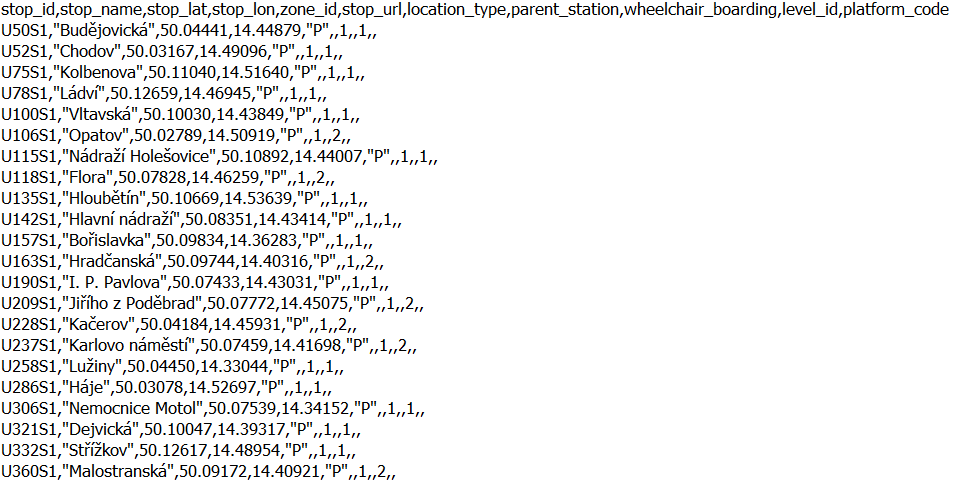
\includegraphics[width=400pt]{./pictures/stops.PNG}
    \caption[Ukázka CSV souboru stops.txt pro PID\_GTFS dataset]{Ukázka CSV souboru stops.txt pro PID\_GTFS dataset}
	\label{fig:stops}              
\end{figure} 
\chapter{Pražská Integrovaná doprava (PID)}
\label{3-teorie-pid}

Pražská integrovaná doprava (PID) je dopravní systém, který zahrnuje jak pozemní
dopravu (tramvaje, železnici, městské a příměstské autobusové linky, lanovou dráhu na Petřín),
tak i tu podzemní (metro). Tento dopravní systém zahrnuje i některé přívozy. 
Systém probíhá integrací společnými přepravními a tarifními podmínkami a jednotným dopravním řešením včetně 
koordinace jízdních řádů. \cite{pid}
\vskip 0.2in
 
\begin{figure}[H] \centering
    
\includegraphics[width=400pt]{./pictures/pid-logo.png}
    \caption[Logo Pražské integrované dopravy]{Logo Pražské integrované dopravy \cite{pid}}
	\label{fig:pid-logo}                                
\end{figure} 

\section{ROPID}

Chod integrace systému zajišťuje Regionální organizátor pražské integrované dopravy (zkráceně ROPID),
což je příspěvková organizace hlavního města Prahy. Jeho úloha je organizační a kontrolní
a ze své práce se odpovídá orgánům samosprávy a státní správy, které jej zabezpečením dopravy pověřily.

\begin{figure}[H] \centering
    
\includegraphics[width=200pt]{./pictures/ropid-logo.jpg}
    \caption[Logo ROPIDu]{Logo ROPIDu \cite{pid}}
	\label{fig:ropid-logo}                                
\end{figure}

ROPID se zabývá vytvářením, rozvíjení, a udržováním systému Pražské integrované dopravy v Praze a okolí,
včetně návazností na jiné systémy jako jsou Integrovaná doprava Plzeňského kraje,
Doprava Ústeckého kraje, Integrovaný dopravní systém Libereckého kraje nebo 
Integrovaná regionální doprava Královéhradeckého a Pardubického kraje.
Taktéž se zabývá vytvářením zásad a standardů dopravní obsluhy a jejich aplikace v závislosti
na dostupných finančních zdrojích a jejich projednání s obcemi, okresními úřady a dopravci.
ROPID výbírá dopravce, uzavírání smluv o závazku veřejné služby jménem města Prahy 
k zajištění provozu PID s dotčenými obcemi, Středočeským krajem a dopravci a kontrola jejich plnění.
Náplní ROPIDu jsou i organizace finančních toků v systému PID, návrh tarifu a jízdného v systému PID a
zajištění jednotnosti informačního systému PID.  \cite{wikipedia-ropid}

\section{Tarifní pásma PID}

Tzv. "tarifní pásma" je rozdělení Pražské integrované dopravy do určitých zón, kde v jednotlivých
zónách platí rozdílná cenové podmínky. Rozdělení tarifních pásem je následující:
P, 0, B, 1, 2, 3, 4, 5, 6, 7, 8, 9. Tarifní pásma P, 0 a B se nacházejí v Praze a územně
se spolu překrývají. Ostatní pásma (1 až 9) se nacházejí ve Středočeském kraji.

Do pásma P jsou zařazeny všechny linky metra, tramvají, městských autobusů, přívozů,
včetně lanové dráhy na Petřín a vybraných železničních stanic a zastávek v centru Prahy.
Pásmo P má dvojnásobnou tarifní hodnotu (tj. je počítáno jako dvě tarifní pásma).
Do pásma 0 jsou zařazeny dojezdové úseky příměstských autobusových linek a vybrané
železniční stanice a zastávky v širší oblasti okolo centra Prahy.
Do pásma B jsou zařazeny úseky příměstských autobusových linek a vybrané 
železniční stanice a zastávky v okrajových částech Prahy. 

Pro pásma nacházející se ve Středočeském kraji jsou zařazeny jednotlivé stanice 
a zastávky příměstských autobusových linek PID a vlaků zařazených do PID. 
Příslušnost stanice nebo zastávky k tarifnímu pásmu je vždy dána jízdním řádem konkrétní linky.\cite{pid}

\begin{figure}[H] \centering
    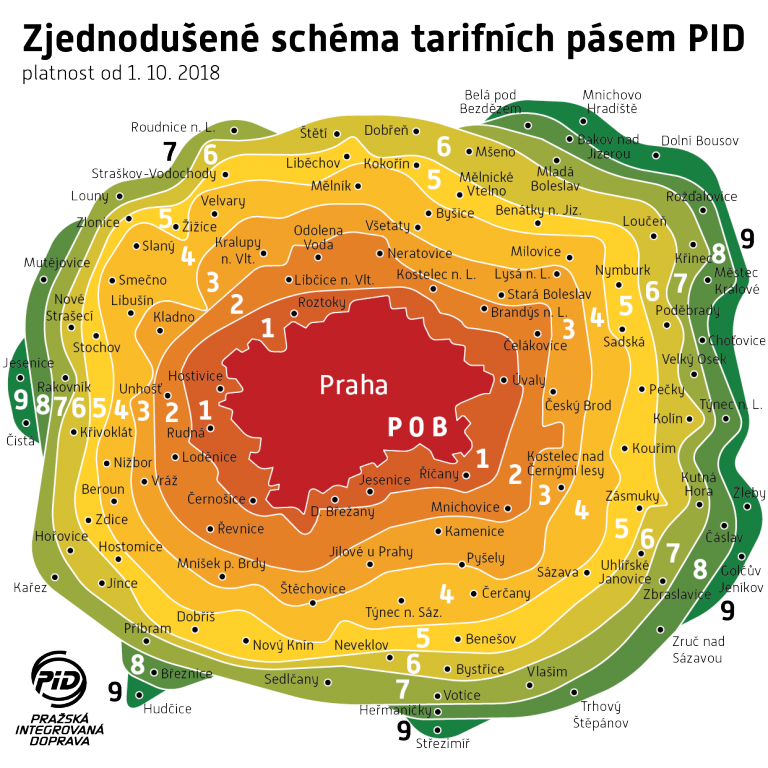
\includegraphics[width=400pt]{./pictures/pasma-schema.png}
    \caption[Schéma tarifních pásem PID]{Schéma tarifních pásem PID \cite{pid}}
	\label{fig:pasma-schema}                                
\end{figure}

\subsection{Tvorba tarifních pásem PID}

Tarifní pásma Pražské integrované dopravy se doposud tvoří manuálně. Zeptal jsem
se tedy paní Ing. Zuzany Šaškové z ROPIDu, která se tvorbou pásem zabývá, jakou metodiku
při tom používá. 

Paní Ing. Šašková používá na úpravu dat software ArcMap od společnosti Esri.
\textit{"Původní myšlenka při tvorbě tarifních pásem byla zohledňovat v mapě 
zastavěná území obce tak, aby je tarifní pásma pokud možno neprotínala,"} od této
myšlenky ustoupila kvůli náročnosti zpracování. \textit{"Dnes mám vytvořeny polygony 
jednotlivých pásem (nikoliv donuty), každé pásmo ručně upravím dle aktuálních změn."} 
V projektu při úpravách nepoužívá žádné sofistikované metody, jenom například obarvení
zastávek a jednotlivých polygonů tarifního pásma stejnou barvou, hraniční zastávek výraznou barvou 
případně pro následné úpravy. \textit{"Když ručně vytvaruji všechny polygony tak, aby procházely 
mezi zastávkami, které mají přiřazené jedno pásmo a skrz zastávky, které mají přiřazená dvě pásma, 
pustím si skript Pythonu, který z polygonů vyřeže donuty jednotlivých tarifních pásem a nakonec je spojí do jedné vrstvy."}

Takto paní Ing. Šašková upravuje tarifní pásma od dubna 2018 při každé úpravě zastávek. 
Zatímco dříve byla důležitá schématická verze mapy, v současnosti se připravuje on-line mapa PID, u které již je zapotřebí 
aby tarifní pásma odpovídala realitě a upravovala se v návaznosti na postup
integrace dalších oblastí Středočeského kraje do PID.

Zde na obrázku \ref{fig:pasma-schema} je uvedena nejstarší dochovaná podoba pásem z dubna roku 2018.
Pro zajímavost si lze všimnout, že v té době tarifní pásmo 7 bylo poslední a všechna pásma tvarově připomínala
spíše tu schématickou verzi.

\begin{figure}[H] \centering
    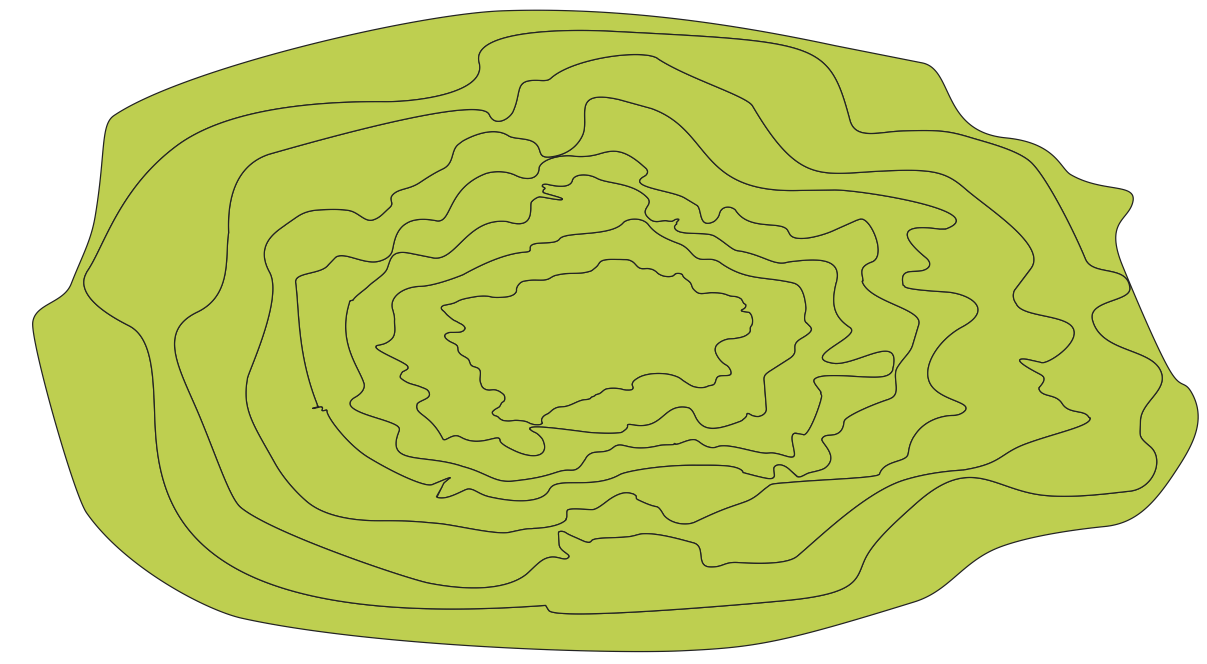
\includegraphics[width=400pt]{./pictures/pasma-nejstarsi.png}
    \caption[Nejstarší dostupná verze tarifních pásem PID]{Nejstarší dostupná verze tarifních pásem PID}
	\label{fig:pasma-schema}                                
\end{figure}




%\chapter{Použité technologie}
\label{4-technologie}

\section{QGIS}

QGIS je profesionální geografický informační systém.
Software je zdarma ke stáhnutí a je tzv. open-source (zdrojový kód je veřejně).
Zdrojový kód je publikován na GitHubu \footnote{webová služba podporující vývoj softwaru za pomoci verzovacího nástroje Git}
a vývojář softwaru může být kdokoliv, avšak potvrzovat a kontrolovat změny můžou jen ověření
přispěvatelé. Software byl vyvíjen v programovacím jazyku C++ a Python (viz \ref{section-python})

\begin{figure}[H] \centering
    
\includegraphics[width=64pt]{./pictures/qgis-logo.png}
    \caption[Logo systému QGIS]{Logo systému QGIS \cite{qgis}}
	\label{fig:qgis-logo}                                
\end{figure}

QGIS je oficiálním projektem nadace OSGeo (Open Source Geospatial Foundation), což je nevládní 
nezisková organizace, jejíž cílem je podporovat a prosazovat společný vývoj otevřených geoinformačních
technologií. Běží na operačních systémech Linux, Unix, Mac OSX, Windows a Android a podporuje
řadu vektorových, rastrových a databázových formátů.

Kromě desktop verze systému QGIS existuje i QGIS Server, který umožňuje publikovat projekty a vrstvy
QGIS jako služby WMS, WMTS, WFS a WCS kompatibilní s OGC (Open Geospatial Consortium - mezinárodní standardizační organizace
o geoprostorových datech a službách). Dále existuje webový klient, kde lze publikovat
QGIS projekty a využívat funkce symboliky a značení. Pro mobilní zařízení tu jsou
různé aplikace jako QField, Input a IntraMaps Roam, se kterými také lze používat QGIS projekty a to 
například přímo v terénu. 

%rozhraní QGIS?

QGIS má jako většina softwarů svou dokumentaci, která je sestavena pomocí nástroje Sphinx. 
Dokumentace je taktéž open-source na GitHubu a upravovat ji může každý. Obsahuje
informace pro obyčejné desktop uživatele systému QGIS, pro přispěvatele dokumentace nebo pro QGIS
vývojáře. V dokumentaci si může uživatel například dočíst informace nebo nápovědu o různých
QGIS nástrojech.

Právě QGIS vývojáři potřebují dokumentaci pro výtváření zautomatizovaných skriptů nebo QGIS zásuvných modulů (pluginů).
Skripty a větší část pluginů jsou vytvářena v programovacím jazyku Python (viz \ref{section-python})
a menší část v programovacím jazyku C++. Instalaci pluginu lze provést z nabídky uvnitř systému QGIS
anebo pomocí ZIP souboru. Pro zobrazení pluginu v QGIS nabídce je potřeba nechat plugin
schválit správci systému QGIS, jestli splňuje všechny povinné aspekty QGIS pluginů.

Součástí systému QGIS je i Model Designer (nebo také Graphical modeler, česky Grafický modelář).
Pomocí Grafického modeláře lze tvořit modely QGIS nástrojů, což jsou uspořádané nástroje do jednoho řetězového postupu.
Pomáhá lépe se v tomto postupu orientovat, měnit vstupy funkcí, pojmenovávat nástroje a jejich parametry,
přidávat komentáře či jednotlivé nástroje seskupovat do skupin. 

\section{Python}
\label{section-python}
Python je moderní, dynamický, skriptovací programovací jazyk s veřejným zdrojovým kódem. 
Je snadný na naučení, lehko čitelný a v současné době velmi populární. Tento programovací jazyk využívají
softwaroví inženýři, matematici, datovi analytici, vědci, účetní a síťoví inženýři.
Dokonce kvůli jednoduchosti tohoto jazyka ho využívají i děti na základních školách.

Důvodů, proč je tento programovací jazyk tak populární, je mnoho. Python je vyšší programovací jazyk,
což znamená lépší srozumitelnost než nižších programovacích jazyků a programy zapsané
ve vyšších jazycích jsou obvykle kratší a lépe čitelné.  Další důvodem je multiplatformovost,
což znamená, že se můžou Pythoní aplikace sestavit a běžet na různých platformách jako 
Windows, Mac či Linux. Komunita Pythonu je obrovská, což je další výhodou tohoto jazyka.
Například jenom v Čechách je mnoho skupin na různých sociálních sítích.
Python má také spoustu knihoven, frameworků a nástrojů, které lidem usnadňují programování.

Podporuje různá programovací paradigmata
\footnote{základní programovací styl, který se liší v pojmech a abstrakcích,
které tvoří jednotlivé prvky programu, a krocích, ze kterých se výpočet skládá  
- objektově orientované, imperativní, procedurální nebo funkcionální \cite{wikipedia-paradigma}} 
jako například objektově orientované, imperativní, procedurální nebo funkcionální.

\begin{figure}[H] \centering
    
\includegraphics[width=260pt]{./pictures/python-logo.png}
    \caption[Logo Pythonu]{Logo Pythonu \cite{python}}
	\label{fig:python-logo}                                
\end{figure} 

\section{PyQt}
Aby aplikaci vytvořenou v Pythonu mohl ovládat člověk, který se neorientuje v programování a ani nechce,
musí se i ke kódu aplikace vytvořit grafické uživatelské rozhraní (GUI). Python má širokou škálu knihoven
pro vytváření GUI jako například Tkinter, wxPython, PySide2 nebo PyQt. Právě PyQt je již standardně 
vestavěný v systému QGIS, tak se zdá jako nejlepší volbou pro tvorbu pluginů.  

PyQt je vazba Pythonu pro aplikační framework Qt vyvinutý společností RiverBank Computing Ltd.
Je k dispozici ve třech verzích: PyQt6 podporuje Qt v6, PyQt5 podporuje Qt v5 a PyQt4 podporuje Qt v4,
avšak PyQt4 s Qt v4 již není podporována. PyQt je multiplatformní a lze nainstalovat na Windows,
macOS, Linux, iOS a Android. \cite{pyqt}

\begin{figure}[H] \centering
    
\includegraphics[width=400pt]{./pictures/pyqt.png}
    \caption[Schéma PyQt Pythonu]{Schéma PyQt}
	\label{fig:pyqt}                                
\end{figure} 

\section{Ostatní}

Pro verzování kódu anebo pro jeho psaní byly použity i další technologie. Diplomová práce by šla tvořit i bez nich,
ale s nimi se zrychloval a usnadňoval její postup.

\subsection{GitHub}

GitHub je služba poskytující internetový hosting pro správu verzí pomocí Git, což je software pro sledování 
změn v libovolné sadě souborů. Tato služba například poskytuje řízení přístupu, sledování chyb, 
správu úkolů nebo nepřetržitou integraci. Základní služby poskytuje zdarma, ale za pokročilé funkce se již musí zaplatit.

\begin{figure}[H] \centering
    
\includegraphics[width=150pt]{./pictures/github.png}
    \caption[Logo GitHubu]{Logo GitHubu \cite{github}}
	\label{fig:github}                                
\end{figure} 

\subsection{PyCharm}

PyCharm je vývojové prostředí vyvinuté firmou JetBrains s.r.o. pro programovací jazyk Python.
Usnadňuje práci s kódem, zvyšuje produktivitu a zpřehledňuje kód například zvýrazněním syntaxe Pythonu.
PyCharm obsahuje širokou kolekci pluginů, které lze doinstalovat a jsou vyvíjeny uživateli.
Skrz PyCharm lze propojit i Git, takže lze snadno kód zálohovat. Jako GitHub základní funkce poskytuje zdarma,
ale profesionální verzi se již musí zaplatit.

\begin{figure}[H] \centering
    
\includegraphics[width=150pt]{./pictures/pycharm.png}
    \caption[Logo PyCharmu]{Logo PyCharmu \cite{pycharm}}
	\label{fig:pycharm}                                
\end{figure} 
 
\chapter{Postup}
\label{5-postup}

\section{Aktualizace pluginu do verze 1.0.0}
Po dokončení pluginu v předmětu Free Software GIS měl plugin veškerou základní 
funkcionalitu, kterou měl mít. Tou bylo načítání GTFS ZIP souboru do QGISu,
rozbalení ZIP souboru, načtení CSV souborů do geodatabázového kontajneru GeoPackage,
vytvoření vektorových vrstev pro soubory \textit{stops.txt} a \textit{shapes.txt},
obarvení vektorové vrty \textit{shapes.txt} a vložení do CSV souborů a vrstev do
\textit{layer tree}.
% vysvětlit layer tree, GeoPackage??

Avšak pro uvedení do "ostrého" provozu musel být plugin více uživatelsky přívětivější.
Proto byl veškerý proces přesunut na pozadí, aby celý QGIS program "nezamrzal" a
mohla se při jeho výpočtech provádět i jiné akce. To se provedlo díky python třídě \textit{QgsTask}
a jejím metodám, které byly zděděny z této třídy. \cite{QgsTask}
% dát sem i ukázku kódu? 

Pro zobrazování procesu během výpočtu byla použita třída \textit{QProgressBar} a její metody.
Zobrazení postupu bylo implementováno do lišty zpráv QGISu spolu s chybovými hláškami.

\begin{figure}[H] \centering
    
\includegraphics[width=400pt]{./pictures/loading.png}
    \caption[ProgressBar]{ProgressBar v liště QGISu}
	\label{fig:ProgressBar v liště QGISu}              
\end{figure}     

% možná přidat code refactorization

\section{Postup 1 - pomocí nástrojů QGIS}

Pro použití QGIS nástrojů v pythoním skriptu je potřeba importovat modul \textit{processing},
který má funkci \textit{run}, do které se vkládají dva parametry. První parametr je ID nástroje
ve formě \textit{stringu} a druhý je \textit{slovník} vstupních parametrů. Vstupní parametry se lze dozvědět
z QGIS dokumentace. \cite{QGIS_docs}

\subsection{Hrubý tvar tarifních pásem}

GTFS obsahuje povinný CSV soubor \textit{stops.txt}. Tento soubor obsahuje mimo
jiných polí také pole \textit{zone\_id}, které bylo při tvorbě tarifních pásem klíčové. 
Pole \textit{zone\_id} má datový typ \textit{string} a znamená, ve kterém tarifním
pásmu daná zastávka leží. Verze GTFS Loaderu 1.0.0 soubor \textit{stops.txt} převádí do vektorové vrstvy
ve formě bodů. Z této bodové vrstvy byla vytvořena vektorová vrstva Voroného 
diagramů nástrojem \textit{Voroného polygony} v programu QGIS. 

Vstupem do tohoto nástroje je vektorová vrstva stops a výstupem jsou právě Voroného polygony.

\begin{figure}[H] \centering
    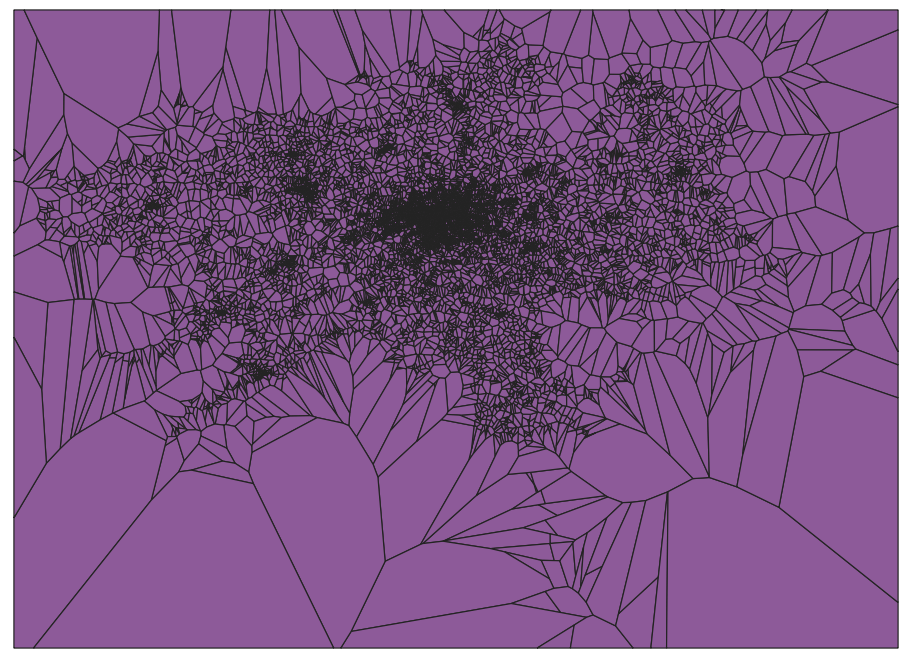
\includegraphics[width=400pt]{./pictures/voronoi-stops.png}
    \caption[Voroného polygony pro všechny zastávky]{Voroného polygony pro všechny zastávky}
	\label{fig:voronoi-stops}              
\end{figure}
  
Pro každé tarifní pásmo byly vybrány zastávky pomocí třídy \textit{QgsVectorLayer}
a její metody \textit{selectByExpression}, která vybírá prvky podle zadaného výrazu ve formě \textit{string}.
Znění zadaného výrazu je následující:

%zjistit, jak lépe přidat části kódu
\textit{zone\_id in "tarifní pásmo" and location\_type = 0}

V zadávaném výrazu figuruje taktéž údaj o poli \textit{location\_type}, což je typ lokace. 
Hodnota nuly (nebo prázdná hodnota) je právě lokace zastávky. 
Třída \textit{QgsVectorLayer} představuje zároveň vektorovou vrstvu, která spravuje
vektorové datové sady a která může být považována jako vstup do nástroje QGIS. % tim chci rict, ze do vstupu nemuze jit string, tzn pouha cesta k vrstve

Pro vybrané zástavky bylo potřeba vybrat ty Voroného polygony, které svou
pozicí dané zastávky protínaly. To bylo provedeno nástrojem \textit{Select by location},
do kterého vstupovala vrstva vybraných zastávek a vrstva Voroného polygonů. Výsledkem tohoto nástroje byla
vektorová vrstva vybraných Voroného polygonů. Jako příklad v obrázku zde budu uvádět tarifní pásmo 2.

\begin{figure}[H] \centering
    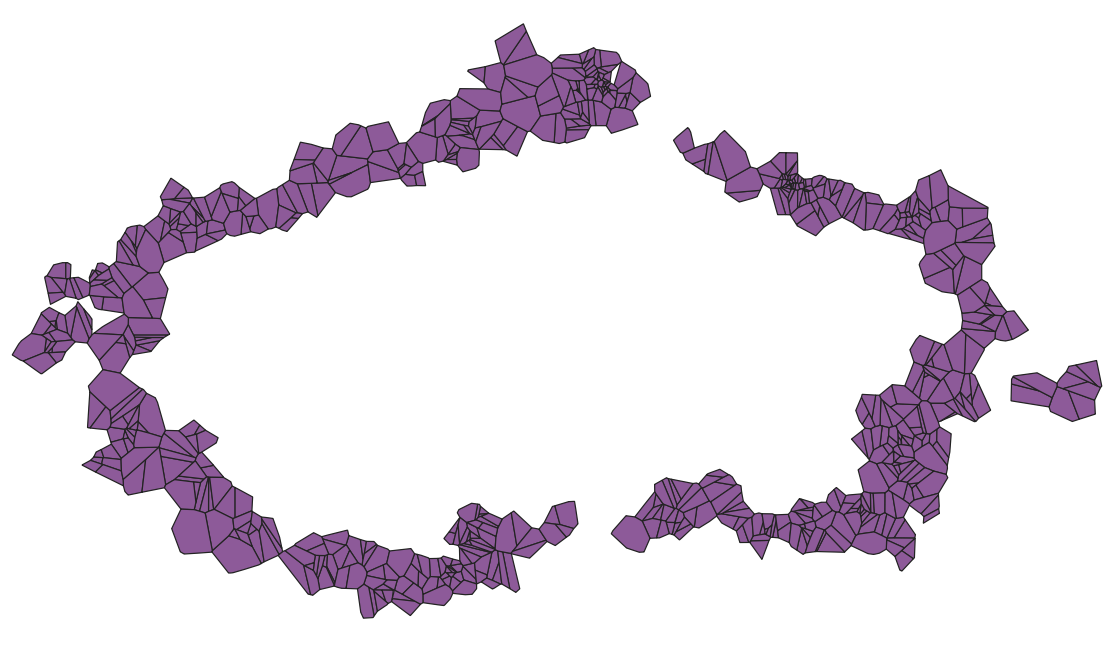
\includegraphics[width=400pt]{./pictures/voronoi-selected.png}
    \caption[Vybrané Voroného polygony pro pásmo 2]{Vybrané Voroného polygony pro pásmo 2}
	\label{fig:voronoi-selected}              
\end{figure}

Tyto polygony byly následně nástrojem \textit{Dissolve} spojeny do jednoho společného polygonu.
Vstupem tohoto nástroje byl výstup nástroje \textit{Select by location} a výstupem byl polygon
s jednou geometrií. 

\begin{figure}[H] \centering
    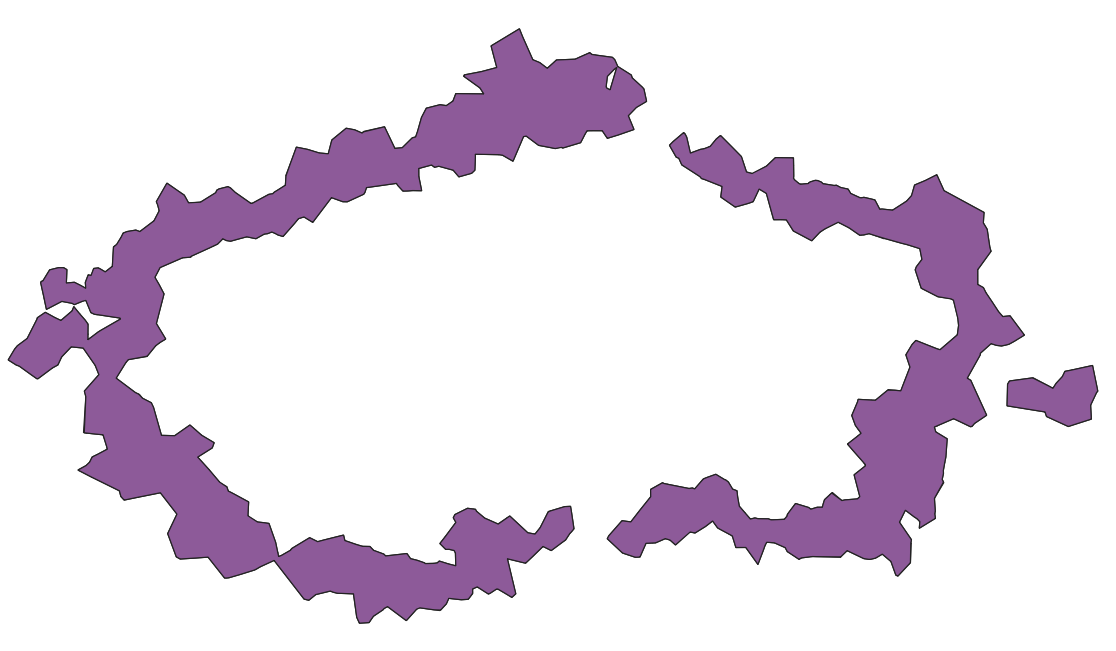
\includegraphics[width=400pt]{./pictures/dissolve.png}
    \caption[Výsledek nástroje Dissolve pro pásmo 2]{Výsledek nástroje Dissolve pro pásmo 2}
	\label{fig:dissolve}              
\end{figure} 

Znázornění tohoto postupu je zobrazeno zde v obrázku \ref{fig:postup-voronoi-P0B}. Toto zobrazení bylo provedeno v Grafickém modeláři
a ukazuje postup pro tarifní pásma P, 0 a B. V následujícím obrázku je \ref{fig:postup-voronoi-1az9} zobrazen postup tarifní pásma 1 až 9.

\begin{figure}[H] \centering
    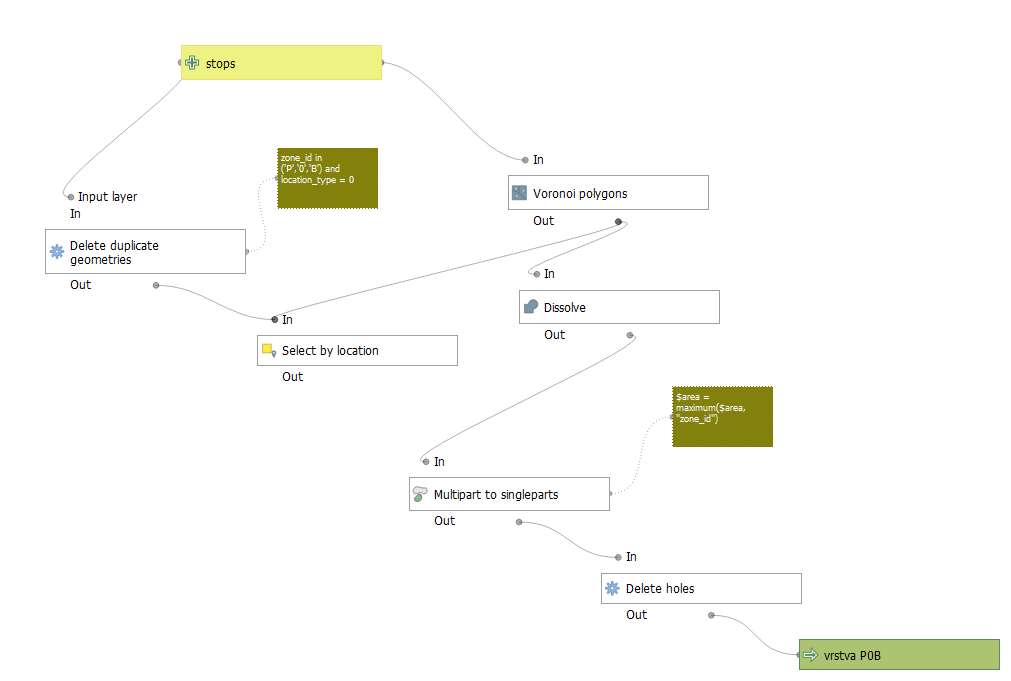
\includegraphics[width=400pt]{./pictures/postup-voronoi-P0B.png}
    \caption[Postup pro tarifní pásma P, 0 a B]{Postup pro tarifní pásma P, 0 a B}
	\label{fig:postup-voronoi-P0B}              
\end{figure}

\begin{figure}[H] \centering
    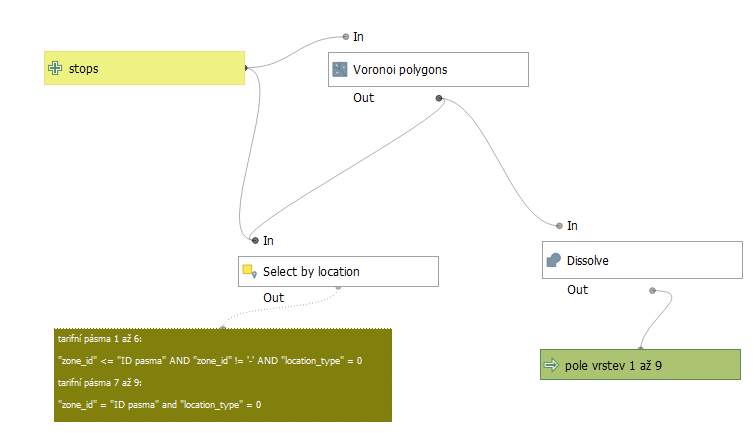
\includegraphics[width=400pt]{./pictures/postup-voronoi-1az9.png}
    \caption[Postup pro tarifní pásma 1 až 9]{Postup pro tarifní pásma 1 až 9}
	\label{fig:postup-voronoi-1az9}              
\end{figure}

\subsection{Vyhlazení tvaru tarifních pásem}

Ze spojených polygonů byla poté vygenerována vektorová vrstva bodů nástrojem
\textit{Extract vertices}, která představovala vrcholy spojených polygonů. Pro tuto vrstvu
bylo vstupem výstup nástroje \textit{Dissolve} a výstupem byl vektorová vrstva bodů 
doplněná o pole (mimo původních polí z vektorové vrstvy \textit{stops}) jako \textit{vertex\_index,
vertex\_part, vertex\_part\_ring, distance} a \textit{angle}.
Hodnoty těchto polí avšak nebyly využity v dalším výpočtu.

\begin{figure}[H] \centering
    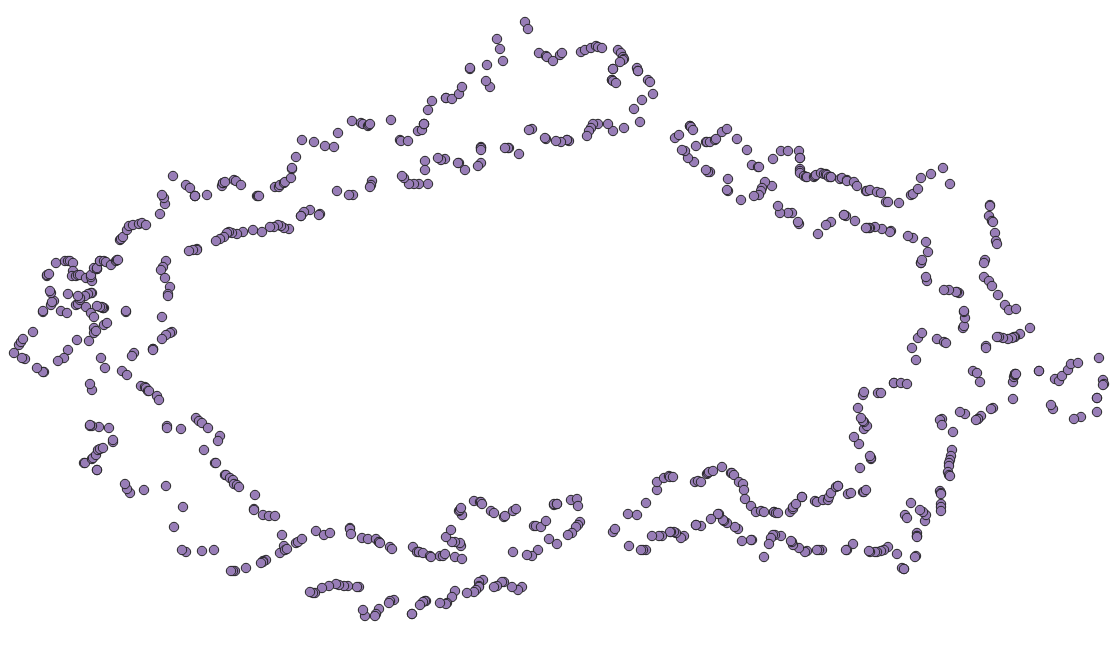
\includegraphics[width=400pt]{./pictures/vertices.png}
    \caption[Výsledek nástroje Extract vertices pro pásmo 2]{Výsledek nástroje Extract vertices pro pásmo 2}
	\label{fig:vertices}              
\end{figure} 

% ------- toto se nejspíš bude předělávat, jiná metoda řešení zastávek na hranici -------
Dále byly s pomocí třídy \textit{QgsVectorLayer} a její metody \textit{selectByExpression} vybrány 
z původní vektorové vrstvy \textit{stops} ty zastávky, které obsahovaly v poli \textit{zone\_id}
hodnotu tarifního pásma 1,2 nebo 2,3. Takové zastávky ležely na hranici pásma a polygon tarifního pásma
měl skrz ně vézt hranici. Z vybraných zastávek byla vytvořena vlastní vektorová vrstva. 
% ------- toto se nejspíš bude předělávat, jiná metoda řešení zastávek na hranici -------

Následně byly spojeny vektorové vrstvy hraniční zastávek, zastávek uvnitř tarifního pásma 2 a
bodů z výstupu nástroje \textit{Extract vertices} nástrojem \textit{Merge vector layers}.
Tyto tři zmiňované vektorové vrstvy byly vstupem do tohoto nástroje a výstupem byla 
vektorová vrstva spojených bodů. 

\begin{figure}[H] \centering
    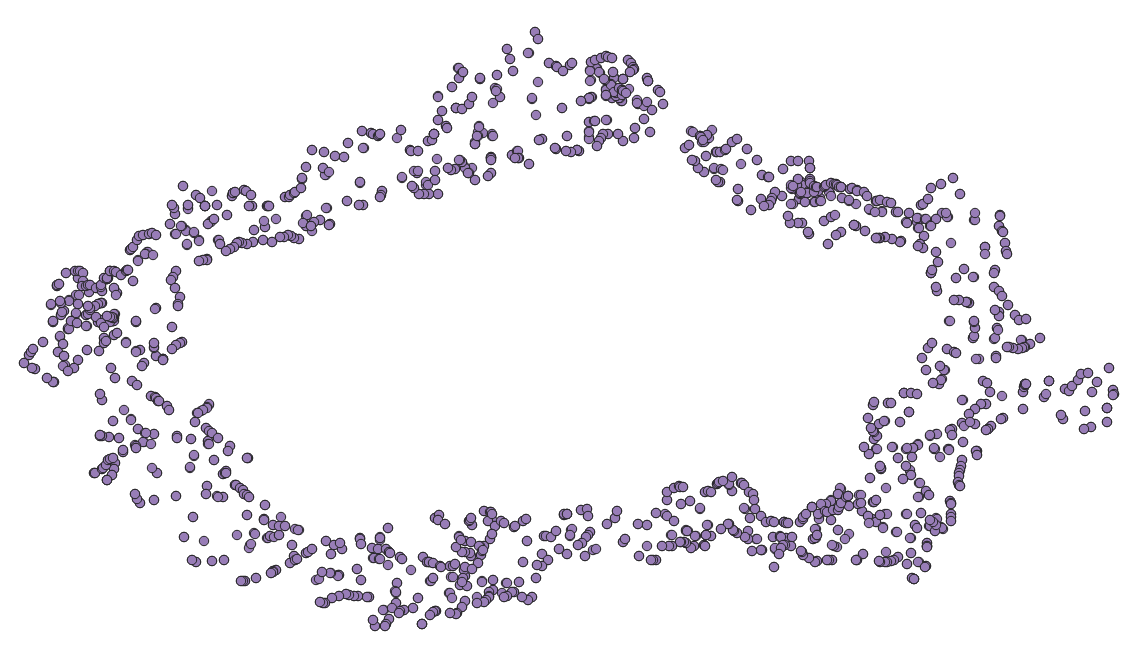
\includegraphics[width=400pt]{./pictures/merged.png}
    \caption[Spojené body třech vektorových vrstev pro pásmo 2]{Spojené body třech vektorových vrstev pro pásmo 2}
	\label{fig:merged}              
\end{figure} 

% Definice konkávní obálky 
Ze spojených bodů byla vytvořena konkávní obálka. To bylo provedeno nástrojem Concave hull (alpha shapes),
který počítá konkávní obálku z vstupních bodů. Vstupem tedy byla vrstva spojených bodů, což byl první parametr
nástroje. Dalším parametrem byl \textit{Práh (Threshold)} s datovým typem \textit{čísla}, který byl volen od 0 do 1,
kdy 0 znamenala maximum konkávní obálky a 1 konvexní obálky. Po několika testovacích spuštění byla 
určena hodnota 0,09 jako nejlepší hodnotou pro tvorbu tarifních pásem. Dalším parametrem bylo \textit{Povolení děr (Allow holes)} 
s datovým typem \textit{boolean}, který byl nastaven na \textit{False}.
Posledním parametrem bylo Rozdělit vícedílnou geometrii na jednotlivé části (Split multipart geometry 
into singlepart geometries) taktéž s datovým typem \textit{boolean}, který byl nastaven na \textit{True}.  
Výstupem byla polygonová vrstva konkávní obálky. 

\begin{figure}[H] \centering
    
\includegraphics[width=400pt]{./pictures/concaveHull.png}
    \caption[Konkávní obálka pro pásmo 2]{Konkávní obálka pro pásmo 2}
	\label{fig:concaveHull}              
\end{figure} 

Z konkávní obálky byla pomocí nástroje Simplify "zjednodušena" geometrie polygonové vrstvy. Tento nástroj
využívá tři druhy zjednodušení vektorové vrstvy: založené na vzdálenosti (algoritmus „Douglas-Peucker“),
založené na ploše (algoritmus „Visvalingam“) a přichytávání geometrií k mřížce.
Pro můj postup byl zvolen první volba zjednodušení, pomocí algoritmu „Douglas-Peucker“.

Algoritmus „Douglas-Peucker“ na rozdíl od ostatních algoritmů neodstraňuje vrcholy nesplňující 
geometrickou podmínku, ale přidává do ní postupně kritické body, které podmínku splnují.
Tento algoritmus je jeden z nejlepších generalizacních algoritmů a je velmi často
implementován v GIS software. \cite{bayer-douglas}

\begin{figure}[H] \centering
    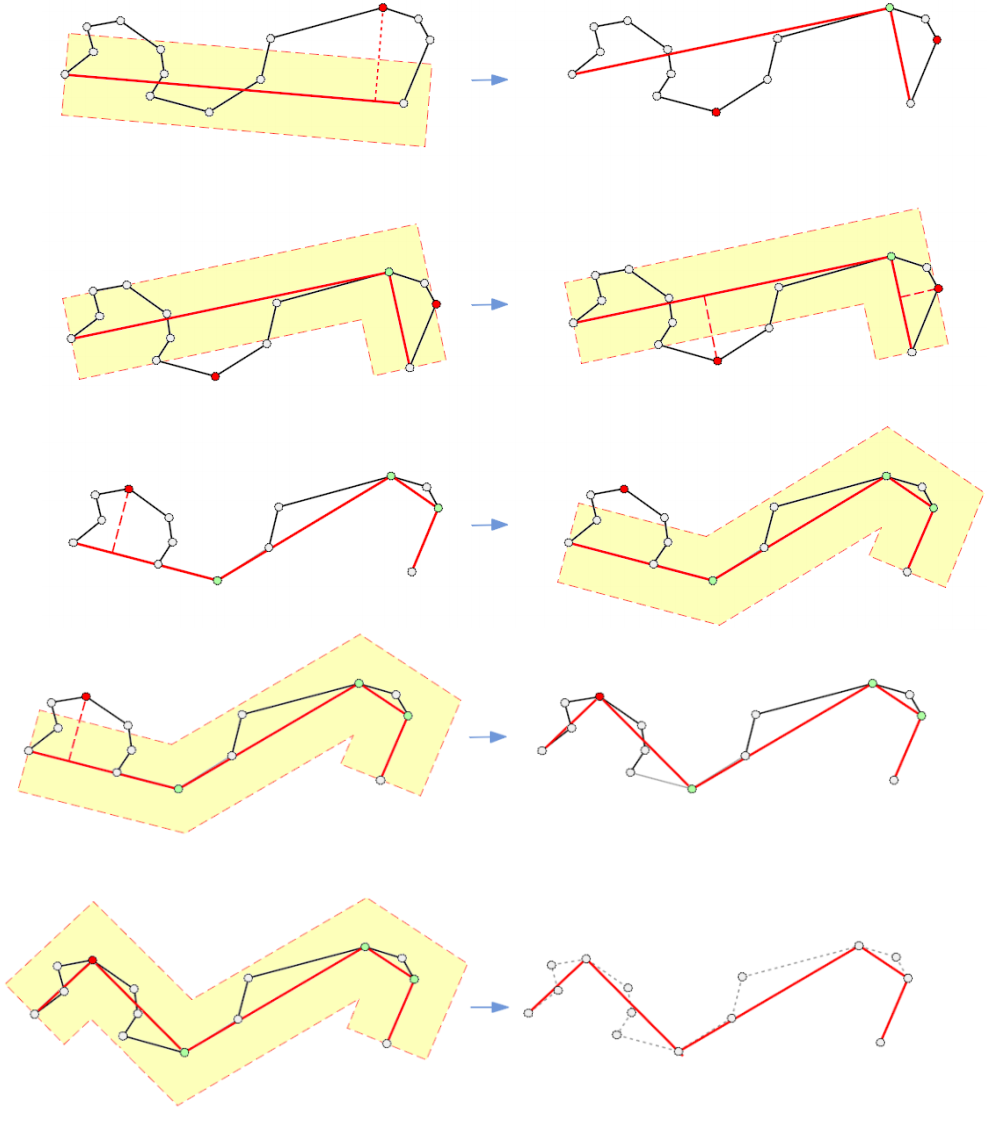
\includegraphics[width=400pt]{./pictures/douglas.png}
    \caption[Znázornění algoritmu „Douglas-Peucker“]{Znázornění algoritmu „Douglas-Peucker“ \cite{bayer-douglas}}
	\label{fig:douglas}              
\end{figure} 

Do nástroje Simplify byl vstupem výsledek nástroje Concave hull (alpha shapes), parametrem byl výběr algoritmu 
a nastavení hodnoty tolerance vzdálenosti. Výstupem byla polygonová vektorová vrstva.

\begin{figure}[H] \centering
    
\includegraphics[width=400pt]{./pictures/simplify.png}
    \caption[Výsledek nástroje Simplify pro pásmo 2]{Výsledek nástroje Simplify pro pásmo 2}
	\label{fig:simplify}                                
\end{figure}

Výstup nástroje Simplify byl vstupem do nástroje Smooth. Tento nástroj vyhlazuje geometrie
liniové nebo polygonové vrstvy pomocí Chaikinova algoritmu.

Chaikin využil fixních poměrů na odříznutí rohů, takže byly všechny rozřezány stejně. 
Při matematickém zápisu postupuje Chaikinova metoda následovně: Dostaneme kontrolní polygon 
\textit{\{P\textsubscript{0}, P\textsubscript{1}, ..., P\textsubscript{n}\}},
tento kontrolní polygon vylepšíme vygenerováním nové posloupnosti řídicích bodů 
\[ \{Q_0, R_0, Q_1, R_1, ...,  Q_{n−1}, R_{n−1}\} \]                                    
kde každá nová dvojice bodů Q\textsubscript{i}, R\textsubscript{i} je třeba brát v poměru \(\frac{1}{4}\)
a \(\frac{3}{4}\) mezi koncovými body segmentu čáry \(\overline{P\textsubscript{i}P\textsubscript{i+1}}\).
\[Q_i = \frac{3}{4}P_i + \frac{1}{4}P_{i+1}\]
\[R_i = \frac{1}{4}P_i + \frac{3}{4}P_{i+1}\]
Tyto 2 nové body lze považovat za nový řídicí polygon - vylepšení původního řídicího polygonu. \cite{chaikin} 

U nástroje Smooth byly zvoleny tři parametry - počet iterací, offset a maximální úhel.
Počet iterací znamená, kolik vyhlazovacích iterací bude použito pro každou geometrii.
Hodnota počtu iterací byla nastavena na 10, což byla maximální volitelná hodnota (pro co nevětší hladkost).
Parametr offset znamená, jak "těsně" vyhlazené geometrie sledují původní geometrie.
Zde byla ponechána výchozí hodnota 0,25. A poslední parametr maximálního úhlu lze použít
k zabránění vyhlazení uzlů s velkými úhly. Zde byla také ponechána výchozí hodnota 180°.
Výstupem nástroje byla polygonová vektorová vrstva.

\begin{figure}[H] \centering
    
\includegraphics[width=400pt]{./pictures/smooth.png}
    \caption[Výsledek nástroje Smooth pro pásmo 2]{Výsledek nástroje Smooth pro pásmo 2}
	\label{fig:smooth}                                
\end{figure}

Zde je souhrně zobrazen postup této části na obrázku \ref{fig:postup-smooth}.

\begin{figure}[H] \centering
    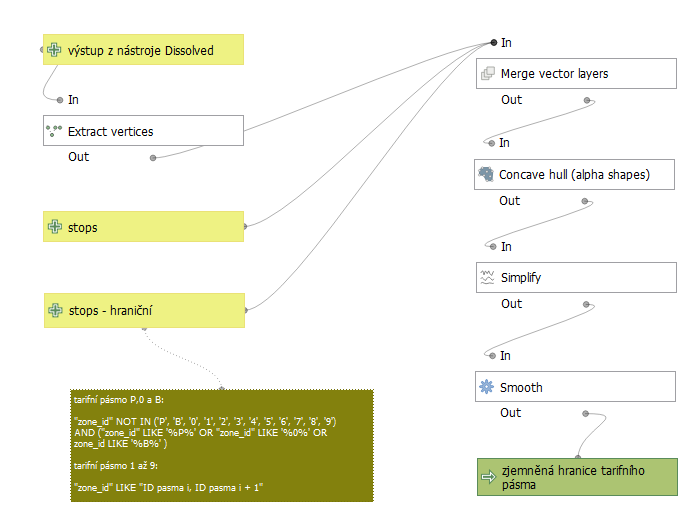
\includegraphics[width=400pt]{./pictures/postup-smooth.png}
    \caption[Postup pro zjemnění tvaru tarfních pásem]{Postup pro zjemnění tvaru tarfních pásem}
	\label{fig:postup-smooth}              
\end{figure}
%\chapter*{Závěr}
\addcontentsline{toc}{chapter}{Závěr}
\markboth{ZÁVĚR}{}
\label{6-zaver}

Primárním cílem této diplomové práce bylo rozšířit plugin systému QGIS 
o automa\-tické vytváření exaktního tvaru tarifních pásem Pražské integrované dopravy, 
jehož referenční podoba je publikována veřejně organizací ROPID.  
Podkladovými daty byl GTFS dataset taktéž zveřejňovaný organizací ROPID.
Mezikrokem k primárnímu cíly bylo zveřejnění pluginu do repozitáře QGIS. Sekundárním cílem bylo vytvořit schématický model pro 
informativní účely, který by se tolik neshodoval s referenční podobou tarifních pásem.

Mezikrok nutný pro pokračování vývoje byl splněn ve formě aktualizace na verzi pluginu 1.0.
V této aktualizaci byly opraveny některé chyby, doplněno uživatelské rozhraní a proces pluginu přeložen na pozadí. 
Následně byl publikován v oficiálním repozitáři systému QGIS s názvem \textit{GTFS Loader}. 
K 12.5.2021 bylo v záložce \textit{Plugins} uvedeno 412 unikátních stáhnutí pluginu.

Implementace tvorby tarifních pásem byla vytvářena jako experimentální verze pluginu 2.0. Výsledek
byl tvořen jako volitelný výstup pluginu ve formě vektorové vrstvy se symbologií jednotlivých tarifních pásem.
Výsledný průběh tarifních pásem byl podobný oficiální verzi publikované veřejně organizací ROPID, ale byl doplněn o tzv. hraniční tarifní pásma,
která pokrývala větší seskupení hraničních zastávek. Pro ostatní nepokryté hraniční zastávky 
se nepodařil najít způsob, jak je napřímo propojit s hranicemi tarifních pásem.

Jak již bylo zmíněno, proces pluginu pro vytváření tarifních pásem nezvládá správně zpracovat hraniční zastávky.
Zároveň v oblastech, kde jsou umístěny zastávky velmi vzácně, vznikají \uv{díry} mezi tarifními pásmy.
Tyto \uv{díry} se ve~snaze pro lepší tvar eliminovaly, ale kvůli tomu vznikl další problém překrývajících se~ta\-rifních pásem.
Každopádně pro lepší tvar je potřeba manuální editace vektorové vrstvy.

Zaměstnanci organizace ROPID bylo dáno pravidlo o nekřížení se intravilánu obce s hranicemi tarifních pásem.
Toto pravidlo mělo mít za následek vyhýbání se~hranic tarifních pásem s většími zastavěnými oblastmi.
Později bylo kvůli obtíž\-nosti s uskutečněním tohoto pravidla upuštěno na přání ze strany pracovníků z~organizace ROPID.
Současně pro realizaci tohoto pravidla by bylo potřeba načítat vektorové vrstvy
dotčených obcí České republiky, což by razantně zvýšilo datovou náročnost pluginu.

Postup navržený v rámci diplomové práce není rozhodně ideální a je na něm co vylepšovat. Předmět úpravy a vylepšení pluginu
se může stát dalším tématem semestrálních či závěrečných prací. Zdrojový kód
je již nyní veřejně přístupný v~repozitáři pluginu s názvem \textit{qgis-gtfs-plugin} ve službe GitHub (odkaz \href{https://github.com/ctu-geoforall-lab/qgis-gtfs-plugin/tree/pid\_zones}
{\underline{zde}}) a kdokoliv k němu může přidávat
návrhy na vylepšení.  



% Vysázení seznamu zkratek
%
\begin{seznamzkratek}{ABCDE}      
	             	                   
      \novazkratka{CSV}
          {CSV}
          {Hodnota oddělená čárkami (Comma-separated values)} 
          
      \novazkratka{DPZ}	
	      {DPZ}
	      {Dálkový průzkum Země}  
          
      \novazkratka{GIS}
	      {GIS}
	      {Geografický informační systém (Geographic information system)}
          
      \novazkratka{GPKG}
	      {GPKG}
	      {Formát dat pro geografický informační systém (GeoPackage)}
          
	  \novazkratka{GUI}	
	      {GUI}
	      {Grafické uživatelské rozhraní (Graphical user interface)}
	               	             
	  \novazkratka{ID}	
	      {ID}
	      {Hodnota jednoznačně určující každý záznam} 	      	     
          
      \novazkratka{URL}
          {URL}
          {Jednotná adresa zdroje (Uniform Resource Locator)}                
          
      \novazkratka{WCS}	
	      {WCS}
	      {Web coverage service}
                                          
	  \novazkratka{WFS}	
	      {WFS}
	      {Web feature service}         
            
	  \novazkratka{WMS}	
	      {WMS}
	      {Webová mapová služba (Web map service)} 	

	  \novazkratka{WMTS}	
	      {WMTS}
	      {Služba webových mapových dlaždic (Web Map Tile Service)} 
          
      \novazkratka{ZIP}
          {ZIP}
          {Formát pro kompresi a archivaci dat} 	
          
	      	      
\end{seznamzkratek}

% Literatura
\nocite{*}
\def\refname{Odkazy}
\bibliographystyle{unsrt}
\bibliography{literatura}


% Začátek příloh
\def\figurename{Figure}%
\prilohy

% Vysázení seznamu příloh
\seznampriloh

%% Vložení souboru s přílohami
%\include{prilohy}

% Konec dokumentu
\end{document}
